\section{Introduction}
\subsection{What is Active Noise Control (ANC)}
\begin{frame}{Introduction}{What is ANC}		
	\begin{columns}
		\begin{column}{0.5\textwidth}
				\begin{itemize}
					\item The basic theory of ANC
					\begin{itemize}
						\item 250 Hz
						\item 2500 Hz 
					\end{itemize}	
				\end{itemize}
			\vspace{-2.5mm}	
		\begin{center}
	 		% This file was created by matlab2tikz.
%
%The latest updates can be retrieved from
%  http://www.mathworks.com/matlabcentral/fileexchange/22022-matlab2tikz-matlab2tikz
%where you can also make suggestions and rate matlab2tikz.
%
\definecolor{mycolor1}{rgb}{0.00000,0.44700,0.74100}%
%
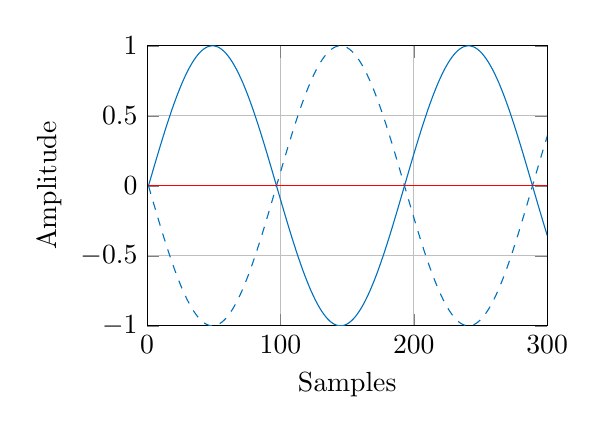
\begin{tikzpicture}

\begin{axis}[%
width=2in,
height=1.4in,
xlabel = {Samples},
ylabel = {Amplitude}, 
scale only axis,
xmin=0,
xmax=300,
xmajorgrids,
ymin=-1,
ymax=1,
ymajorgrids,
axis background/.style={fill=white}
]
\addplot [color=mycolor1,solid,forget plot]
  table[row sep=crcr]{%
1	0\\
2	0.0327190828217761\\
3	0.0654031292301431\\
4	0.0980171403295606\\
5	0.130526192220052\\
6	0.162895473394589\\
7	0.195090322016128\\
8	0.227076263034373\\
9	0.258819045102521\\
10	0.290284677254462\\
11	0.321439465303162\\
12	0.352250047921233\\
13	0.38268343236509\\
14	0.412707029804395\\
15	0.442288690219001\\
16	0.471396736825998\\
17	0.5\\
18	0.528067850650368\\
19	0.555570233019602\\
20	0.582477696867802\\
21	0.608761429008721\\
22	0.634393284163645\\
23	0.659345815100069\\
24	0.683592302022871\\
25	0.707106781186547\\
26	0.729864072697836\\
27	0.751839807478977\\
28	0.773010453362737\\
29	0.793353340291235\\
30	0.812846684591615\\
31	0.831469612302545\\
32	0.849202181526579\\
33	0.866025403784439\\
34	0.881921264348355\\
35	0.896872741532688\\
36	0.910863824921176\\
37	0.923879532511287\\
38	0.935905926757326\\
39	0.946930129495106\\
40	0.956940335732209\\
41	0.965925826289068\\
42	0.973876979277334\\
43	0.98078528040323\\
44	0.986643332084879\\
45	0.99144486137381\\
46	0.995184726672197\\
47	0.997858923238603\\
48	0.999464587476366\\
49	1\\
50	0.999464587476366\\
51	0.997858923238603\\
52	0.995184726672197\\
53	0.99144486137381\\
54	0.986643332084879\\
55	0.980785280403231\\
56	0.973876979277334\\
57	0.965925826289068\\
58	0.956940335732209\\
59	0.946930129495106\\
60	0.935905926757326\\
61	0.923879532511287\\
62	0.910863824921176\\
63	0.896872741532688\\
64	0.881921264348355\\
65	0.866025403784439\\
66	0.849202181526579\\
67	0.831469612302545\\
68	0.812846684591615\\
69	0.793353340291235\\
70	0.773010453362737\\
71	0.751839807478978\\
72	0.729864072697836\\
73	0.707106781186548\\
74	0.683592302022872\\
75	0.659345815100069\\
76	0.634393284163645\\
77	0.60876142900872\\
78	0.582477696867802\\
79	0.555570233019603\\
80	0.528067850650368\\
81	0.5\\
82	0.471396736825998\\
83	0.442288690219002\\
84	0.412707029804395\\
85	0.38268343236509\\
86	0.352250047921233\\
87	0.321439465303161\\
88	0.290284677254463\\
89	0.258819045102521\\
90	0.227076263034374\\
91	0.195090322016129\\
92	0.162895473394589\\
93	0.130526192220052\\
94	0.0980171403295608\\
95	0.0654031292301431\\
96	0.0327190828217764\\
97	1.22464679914735e-16\\
98	-0.0327190828217758\\
99	-0.0654031292301424\\
100	-0.0980171403295606\\
101	-0.130526192220051\\
102	-0.162895473394588\\
103	-0.195090322016128\\
104	-0.227076263034373\\
105	-0.258819045102521\\
106	-0.290284677254462\\
107	-0.321439465303162\\
108	-0.352250047921233\\
109	-0.382683432365089\\
110	-0.412707029804395\\
111	-0.442288690219001\\
112	-0.471396736825998\\
113	-0.5\\
114	-0.528067850650368\\
115	-0.555570233019602\\
116	-0.582477696867802\\
117	-0.608761429008721\\
118	-0.634393284163645\\
119	-0.659345815100069\\
120	-0.683592302022871\\
121	-0.707106781186548\\
122	-0.729864072697836\\
123	-0.751839807478977\\
124	-0.773010453362737\\
125	-0.793353340291235\\
126	-0.812846684591615\\
127	-0.831469612302545\\
128	-0.849202181526579\\
129	-0.866025403784438\\
130	-0.881921264348354\\
131	-0.896872741532688\\
132	-0.910863824921175\\
133	-0.923879532511287\\
134	-0.935905926757326\\
135	-0.946930129495106\\
136	-0.956940335732209\\
137	-0.965925826289068\\
138	-0.973876979277334\\
139	-0.98078528040323\\
140	-0.986643332084879\\
141	-0.99144486137381\\
142	-0.995184726672197\\
143	-0.997858923238603\\
144	-0.999464587476366\\
145	-1\\
146	-0.999464587476366\\
147	-0.997858923238604\\
148	-0.995184726672197\\
149	-0.99144486137381\\
150	-0.986643332084879\\
151	-0.98078528040323\\
152	-0.973876979277334\\
153	-0.965925826289068\\
154	-0.956940335732209\\
155	-0.946930129495105\\
156	-0.935905926757326\\
157	-0.923879532511287\\
158	-0.910863824921176\\
159	-0.896872741532688\\
160	-0.881921264348355\\
161	-0.866025403784439\\
162	-0.849202181526579\\
163	-0.831469612302545\\
164	-0.812846684591615\\
165	-0.793353340291236\\
166	-0.773010453362737\\
167	-0.751839807478978\\
168	-0.729864072697836\\
169	-0.707106781186548\\
170	-0.683592302022872\\
171	-0.659345815100069\\
172	-0.634393284163646\\
173	-0.60876142900872\\
174	-0.582477696867802\\
175	-0.555570233019603\\
176	-0.528067850650368\\
177	-0.5\\
178	-0.471396736825998\\
179	-0.442288690219002\\
180	-0.412707029804395\\
181	-0.38268343236509\\
182	-0.352250047921234\\
183	-0.321439465303162\\
184	-0.290284677254463\\
185	-0.258819045102522\\
186	-0.227076263034374\\
187	-0.195090322016129\\
188	-0.162895473394589\\
189	-0.130526192220052\\
190	-0.0980171403295605\\
191	-0.0654031292301437\\
192	-0.0327190828217766\\
193	-2.44929359829471e-16\\
194	0.0327190828217752\\
195	0.0654031292301423\\
196	0.0980171403295609\\
197	0.13052619222005\\
198	0.162895473394589\\
199	0.195090322016128\\
200	0.227076263034373\\
201	0.25881904510252\\
202	0.290284677254462\\
203	0.321439465303161\\
204	0.352250047921233\\
205	0.382683432365089\\
206	0.412707029804394\\
207	0.442288690219002\\
208	0.471396736825997\\
209	0.5\\
210	0.528067850650368\\
211	0.555570233019601\\
212	0.582477696867802\\
213	0.608761429008721\\
214	0.634393284163645\\
215	0.659345815100068\\
216	0.683592302022872\\
217	0.707106781186547\\
218	0.729864072697836\\
219	0.751839807478978\\
220	0.773010453362736\\
221	0.793353340291235\\
222	0.812846684591615\\
223	0.831469612302545\\
224	0.849202181526578\\
225	0.866025403784438\\
226	0.881921264348355\\
227	0.896872741532689\\
228	0.910863824921175\\
229	0.923879532511287\\
230	0.935905926757326\\
231	0.946930129495105\\
232	0.956940335732209\\
233	0.965925826289068\\
234	0.973876979277334\\
235	0.98078528040323\\
236	0.986643332084879\\
237	0.99144486137381\\
238	0.995184726672197\\
239	0.997858923238603\\
240	0.999464587476366\\
241	1\\
242	0.999464587476366\\
243	0.997858923238603\\
244	0.995184726672197\\
245	0.99144486137381\\
246	0.986643332084879\\
247	0.98078528040323\\
248	0.973876979277334\\
249	0.965925826289068\\
250	0.956940335732209\\
251	0.946930129495106\\
252	0.935905926757325\\
253	0.923879532511287\\
254	0.910863824921176\\
255	0.896872741532688\\
256	0.881921264348355\\
257	0.866025403784439\\
258	0.849202181526579\\
259	0.831469612302547\\
260	0.812846684591615\\
261	0.793353340291235\\
262	0.773010453362738\\
263	0.751839807478978\\
264	0.729864072697835\\
265	0.707106781186548\\
266	0.683592302022871\\
267	0.65934581510007\\
268	0.634393284163647\\
269	0.608761429008721\\
270	0.582477696867803\\
271	0.555570233019602\\
272	0.528067850650369\\
273	0.5\\
274	0.471396736825998\\
275	0.442288690219001\\
276	0.412707029804396\\
277	0.382683432365091\\
278	0.352250047921233\\
279	0.321439465303162\\
280	0.290284677254463\\
281	0.258819045102523\\
282	0.227076263034374\\
283	0.195090322016128\\
284	0.162895473394589\\
285	0.130526192220053\\
286	0.0980171403295624\\
287	0.0654031292301438\\
288	0.0327190828217758\\
289	3.67394039744206e-16\\
290	-0.0327190828217751\\
291	-0.0654031292301431\\
292	-0.0980171403295617\\
293	-0.13052619222005\\
294	-0.162895473394588\\
295	-0.195090322016126\\
296	-0.227076263034373\\
297	-0.25881904510252\\
298	-0.290284677254461\\
299	-0.32143946530316\\
300	-0.352250047921234\\
301	-0.38268343236509\\
302	-0.412707029804394\\
303	-0.442288690219\\
304	-0.471396736825996\\
305	-0.500000000000001\\
306	-0.528067850650368\\
307	-0.555570233019602\\
308	-0.582477696867801\\
309	-0.608761429008722\\
310	-0.634393284163645\\
311	-0.659345815100069\\
312	-0.68359230202287\\
313	-0.707106781186547\\
314	-0.729864072697835\\
315	-0.751839807478977\\
316	-0.773010453362736\\
317	-0.793353340291235\\
318	-0.812846684591614\\
319	-0.831469612302545\\
320	-0.849202181526578\\
321	-0.866025403784438\\
322	-0.881921264348355\\
323	-0.896872741532689\\
324	-0.910863824921176\\
325	-0.923879532511286\\
326	-0.935905926757325\\
327	-0.946930129495105\\
328	-0.956940335732209\\
329	-0.965925826289068\\
330	-0.973876979277333\\
331	-0.98078528040323\\
332	-0.986643332084879\\
333	-0.99144486137381\\
334	-0.995184726672197\\
335	-0.997858923238603\\
336	-0.999464587476366\\
337	-1\\
338	-0.999464587476366\\
339	-0.997858923238604\\
340	-0.995184726672197\\
341	-0.99144486137381\\
342	-0.986643332084879\\
343	-0.980785280403231\\
344	-0.973876979277334\\
345	-0.965925826289068\\
346	-0.956940335732209\\
347	-0.946930129495106\\
348	-0.935905926757326\\
349	-0.923879532511287\\
350	-0.910863824921176\\
351	-0.896872741532688\\
352	-0.881921264348356\\
353	-0.866025403784439\\
354	-0.849202181526579\\
355	-0.831469612302546\\
356	-0.812846684591616\\
357	-0.793353340291236\\
358	-0.773010453362738\\
359	-0.751839807478977\\
360	-0.729864072697836\\
361	-0.707106781186548\\
362	-0.683592302022871\\
363	-0.65934581510007\\
364	-0.634393284163645\\
365	-0.608761429008721\\
366	-0.582477696867803\\
367	-0.555570233019604\\
368	-0.528067850650367\\
369	-0.500000000000001\\
370	-0.471396736825998\\
371	-0.442288690219002\\
372	-0.412707029804395\\
373	-0.382683432365091\\
374	-0.352250047921235\\
375	-0.321439465303162\\
376	-0.290284677254464\\
377	-0.258819045102521\\
378	-0.227076263034376\\
379	-0.195090322016128\\
380	-0.162895473394591\\
381	-0.130526192220053\\
382	-0.0980171403295608\\
383	-0.0654031292301439\\
384	-0.0327190828217795\\
385	-4.89858719658941e-16\\
386	0.032719082821775\\
387	0.0654031292301412\\
388	0.0980171403295598\\
389	0.13052619222005\\
390	0.162895473394588\\
391	0.195090322016129\\
392	0.227076263034373\\
393	0.258819045102518\\
394	0.290284677254461\\
395	0.321439465303161\\
396	0.352250047921232\\
397	0.38268343236509\\
398	0.412707029804394\\
399	0.442288690219\\
400	0.471396736825999\\
401	0.499999999999999\\
402	0.528067850650366\\
403	0.555570233019602\\
404	0.582477696867802\\
405	0.608761429008719\\
406	0.634393284163646\\
407	0.659345815100068\\
408	0.683592302022871\\
409	0.707106781186547\\
410	0.729864072697835\\
411	0.751839807478977\\
412	0.773010453362735\\
413	0.793353340291236\\
414	0.812846684591614\\
415	0.831469612302544\\
416	0.849202181526578\\
417	0.866025403784439\\
418	0.881921264348354\\
419	0.896872741532688\\
420	0.910863824921175\\
421	0.923879532511286\\
422	0.935905926757326\\
423	0.946930129495105\\
424	0.956940335732208\\
425	0.965925826289068\\
426	0.973876979277333\\
427	0.98078528040323\\
428	0.986643332084879\\
429	0.99144486137381\\
430	0.995184726672197\\
431	0.997858923238604\\
432	0.999464587476366\\
433	1\\
434	0.999464587476366\\
435	0.997858923238603\\
436	0.995184726672197\\
437	0.99144486137381\\
438	0.986643332084879\\
439	0.980785280403231\\
440	0.973876979277334\\
441	0.965925826289069\\
442	0.956940335732209\\
443	0.946930129495106\\
444	0.935905926757326\\
445	0.923879532511287\\
446	0.910863824921177\\
447	0.896872741532689\\
448	0.881921264348356\\
449	0.866025403784439\\
450	0.849202181526579\\
451	0.831469612302546\\
452	0.812846684591617\\
453	0.793353340291234\\
454	0.773010453362738\\
455	0.751839807478979\\
456	0.729864072697836\\
457	0.707106781186549\\
458	0.683592302022873\\
459	0.659345815100068\\
460	0.634393284163647\\
461	0.608761429008723\\
462	0.582477696867802\\
463	0.555570233019603\\
464	0.528067850650369\\
465	0.5\\
466	0.471396736825998\\
467	0.442288690219003\\
468	0.412707029804397\\
469	0.382683432365091\\
470	0.352250047921235\\
471	0.321439465303164\\
472	0.290284677254462\\
473	0.258819045102523\\
474	0.227076263034376\\
475	0.19509032201613\\
476	0.162895473394589\\
477	0.130526192220053\\
478	0.0980171403295609\\
479	0.0654031292301458\\
480	0.0327190828217761\\
481	-1.16403343982657e-15\\
482	-0.0327190828217784\\
483	-0.0654031292301428\\
484	-0.0980171403295579\\
485	-0.130526192220055\\
486	-0.16289547339459\\
487	-0.195090322016127\\
488	-0.227076263034373\\
489	-0.258819045102523\\
490	-0.290284677254461\\
491	-0.321439465303161\\
492	-0.352250047921237\\
493	-0.382683432365091\\
494	-0.412707029804397\\
495	-0.442288690219001\\
496	-0.471396736825999\\
497	-0.499999999999999\\
498	-0.528067850650368\\
499	-0.5555702330196\\
500	-0.582477696867804\\
501	-0.608761429008723\\
502	-0.634393284163646\\
503	-0.65934581510007\\
504	-0.683592302022873\\
505	-0.707106781186548\\
506	-0.729864072697834\\
507	-0.751839807478977\\
508	-0.773010453362737\\
509	-0.793353340291236\\
510	-0.812846684591616\\
511	-0.831469612302547\\
512	-0.849202181526579\\
513	-0.866025403784439\\
514	-0.881921264348355\\
515	-0.896872741532688\\
516	-0.910863824921176\\
517	-0.923879532511286\\
518	-0.935905926757326\\
519	-0.946930129495107\\
520	-0.956940335732209\\
521	-0.965925826289068\\
522	-0.973876979277334\\
523	-0.980785280403231\\
524	-0.986643332084879\\
525	-0.99144486137381\\
526	-0.995184726672197\\
527	-0.997858923238604\\
528	-0.999464587476366\\
529	-1\\
530	-0.999464587476366\\
531	-0.997858923238603\\
532	-0.995184726672197\\
533	-0.991444861373811\\
534	-0.986643332084879\\
535	-0.98078528040323\\
536	-0.973876979277333\\
537	-0.965925826289069\\
538	-0.956940335732208\\
539	-0.946930129495105\\
540	-0.935905926757326\\
541	-0.923879532511287\\
542	-0.910863824921175\\
543	-0.896872741532689\\
544	-0.881921264348355\\
545	-0.866025403784438\\
546	-0.849202181526578\\
547	-0.831469612302544\\
548	-0.812846684591615\\
549	-0.793353340291234\\
550	-0.773010453362736\\
551	-0.751839807478978\\
552	-0.729864072697837\\
553	-0.707106781186546\\
554	-0.683592302022869\\
555	-0.659345815100069\\
556	-0.634393284163644\\
557	-0.608761429008719\\
558	-0.582477696867802\\
559	-0.555570233019604\\
560	-0.528067850650369\\
561	-0.5\\
562	-0.471396736826\\
563	-0.442288690218999\\
564	-0.412707029804392\\
565	-0.382683432365089\\
566	-0.352250047921232\\
567	-0.321439465303162\\
568	-0.290284677254462\\
569	-0.258819045102519\\
570	-0.227076263034374\\
571	-0.195090322016132\\
572	-0.162895473394588\\
573	-0.13052619222005\\
574	-0.098017140329561\\
575	-0.0654031292301424\\
576	-0.0327190828217744\\
577	-7.34788079488412e-16\\
578	0.0327190828217765\\
579	0.0654031292301409\\
580	0.0980171403295595\\
581	0.130526192220055\\
582	0.16289547339459\\
583	0.19509032201613\\
584	0.227076263034376\\
585	0.258819045102521\\
586	0.290284677254461\\
587	0.321439465303164\\
588	0.352250047921234\\
589	0.382683432365088\\
590	0.412707029804397\\
591	0.442288690219005\\
592	0.471396736825999\\
593	0.500000000000002\\
594	0.528067850650368\\
595	0.555570233019603\\
596	0.582477696867804\\
597	0.608761429008717\\
598	0.634393284163646\\
599	0.65934581510007\\
600	0.683592302022871\\
601	0.707106781186548\\
602	0.729864072697836\\
603	0.751839807478977\\
604	0.773010453362737\\
605	0.793353340291236\\
606	0.812846684591614\\
607	0.831469612302545\\
608	0.849202181526579\\
609	0.866025403784439\\
610	0.881921264348356\\
611	0.896872741532688\\
612	0.910863824921175\\
613	0.923879532511286\\
614	0.935905926757326\\
615	0.946930129495105\\
616	0.956940335732208\\
617	0.965925826289069\\
618	0.973876979277334\\
619	0.980785280403231\\
620	0.986643332084879\\
621	0.99144486137381\\
622	0.995184726672197\\
623	0.997858923238603\\
624	0.999464587476366\\
625	1\\
626	0.999464587476366\\
627	0.997858923238604\\
628	0.995184726672197\\
629	0.99144486137381\\
630	0.986643332084879\\
631	0.98078528040323\\
632	0.973876979277334\\
633	0.965925826289069\\
634	0.956940335732209\\
635	0.946930129495105\\
636	0.935905926757325\\
637	0.923879532511286\\
638	0.910863824921176\\
639	0.896872741532689\\
640	0.881921264348354\\
641	0.866025403784438\\
642	0.84920218152658\\
643	0.831469612302546\\
644	0.812846684591613\\
645	0.793353340291235\\
646	0.773010453362736\\
647	0.751839807478978\\
648	0.729864072697835\\
649	0.707106781186546\\
650	0.683592302022872\\
651	0.659345815100069\\
652	0.634393284163644\\
653	0.608761429008721\\
654	0.582477696867802\\
655	0.555570233019601\\
656	0.528067850650369\\
657	0.5\\
658	0.471396736825997\\
659	0.442288690219003\\
660	0.412707029804395\\
661	0.382683432365089\\
662	0.352250047921232\\
663	0.321439465303159\\
664	0.290284677254459\\
665	0.258819045102523\\
666	0.227076263034374\\
667	0.195090322016125\\
668	0.162895473394591\\
669	0.130526192220053\\
670	0.0980171403295611\\
671	0.0654031292301425\\
672	0.0327190828217745\\
673	8.57252759403147e-16\\
674	-0.0327190828217764\\
675	-0.0654031292301444\\
676	-0.0980171403295594\\
677	-0.130526192220048\\
678	-0.16289547339459\\
679	-0.195090322016127\\
680	-0.227076263034373\\
681	-0.258819045102521\\
682	-0.290284677254464\\
683	-0.321439465303161\\
684	-0.352250047921234\\
685	-0.382683432365091\\
686	-0.412707029804394\\
687	-0.442288690219001\\
688	-0.471396736825995\\
689	-0.500000000000002\\
690	-0.528067850650371\\
691	-0.555570233019603\\
692	-0.582477696867801\\
693	-0.608761429008723\\
694	-0.634393284163646\\
695	-0.659345815100067\\
696	-0.68359230202287\\
697	-0.707106781186548\\
698	-0.729864072697836\\
699	-0.751839807478979\\
700	-0.773010453362737\\
701	-0.793353340291236\\
702	-0.812846684591616\\
703	-0.831469612302545\\
704	-0.849202181526579\\
705	-0.866025403784439\\
706	-0.881921264348355\\
707	-0.896872741532688\\
708	-0.910863824921176\\
709	-0.923879532511288\\
710	-0.935905926757326\\
711	-0.946930129495106\\
712	-0.956940335732209\\
713	-0.965925826289068\\
714	-0.973876979277334\\
715	-0.98078528040323\\
716	-0.986643332084879\\
717	-0.991444861373811\\
718	-0.995184726672197\\
719	-0.997858923238603\\
720	-0.999464587476366\\
721	-1\\
722	-0.999464587476366\\
723	-0.997858923238604\\
724	-0.995184726672197\\
725	-0.99144486137381\\
726	-0.986643332084879\\
727	-0.98078528040323\\
728	-0.973876979277333\\
729	-0.965925826289069\\
730	-0.956940335732209\\
731	-0.946930129495105\\
732	-0.935905926757326\\
733	-0.923879532511288\\
734	-0.910863824921176\\
735	-0.896872741532688\\
736	-0.881921264348355\\
737	-0.866025403784438\\
738	-0.849202181526578\\
739	-0.831469612302546\\
740	-0.812846684591615\\
741	-0.793353340291237\\
742	-0.773010453362738\\
743	-0.751839807478975\\
744	-0.729864072697835\\
745	-0.707106781186549\\
746	-0.683592302022869\\
747	-0.659345815100069\\
748	-0.634393284163647\\
749	-0.608761429008722\\
750	-0.582477696867802\\
751	-0.555570233019604\\
752	-0.528067850650366\\
753	-0.499999999999997\\
754	-0.471396736825997\\
755	-0.442288690219\\
756	-0.412707029804392\\
757	-0.382683432365089\\
758	-0.352250047921232\\
759	-0.321439465303159\\
760	-0.290284677254466\\
761	-0.25881904510252\\
762	-0.227076263034368\\
763	-0.195090322016129\\
764	-0.162895473394588\\
765	-0.13052619222005\\
766	-0.0980171403295612\\
767	-0.0654031292301426\\
768	-0.0327190828217746\\
769	-9.79717439317883e-16\\
770	0.0327190828217798\\
771	0.0654031292301478\\
772	0.0980171403295593\\
773	0.130526192220055\\
774	0.162895473394586\\
775	0.195090322016127\\
776	0.227076263034373\\
777	0.258819045102518\\
778	0.29028467725446\\
779	0.321439465303164\\
780	0.352250047921234\\
781	0.382683432365091\\
782	0.412707029804397\\
783	0.442288690219001\\
784	0.471396736825998\\
785	0.500000000000002\\
786	0.528067850650365\\
787	0.5555702330196\\
788	0.582477696867806\\
789	0.60876142900872\\
790	0.634393284163646\\
791	0.65934581510007\\
792	0.68359230202287\\
793	0.707106781186547\\
794	0.729864072697836\\
795	0.751839807478976\\
796	0.773010453362737\\
797	0.793353340291238\\
798	0.812846684591614\\
799	0.831469612302547\\
800	0.849202181526577\\
801	0.866025403784437\\
802	0.881921264348354\\
803	0.896872741532687\\
804	0.910863824921175\\
805	0.923879532511286\\
806	0.935905926757326\\
807	0.946930129495106\\
808	0.956940335732209\\
809	0.965925826289067\\
810	0.973876979277334\\
811	0.980785280403231\\
812	0.986643332084878\\
813	0.99144486137381\\
814	0.995184726672197\\
815	0.997858923238603\\
816	0.999464587476366\\
817	1\\
818	0.999464587476366\\
819	0.997858923238604\\
820	0.995184726672197\\
821	0.991444861373811\\
822	0.986643332084879\\
823	0.98078528040323\\
824	0.973876979277334\\
825	0.965925826289068\\
826	0.956940335732208\\
827	0.946930129495107\\
828	0.935905926757326\\
829	0.923879532511287\\
830	0.910863824921177\\
831	0.896872741532689\\
832	0.881921264348355\\
833	0.866025403784439\\
834	0.849202181526578\\
835	0.831469612302544\\
836	0.812846684591615\\
837	0.793353340291235\\
838	0.773010453362736\\
839	0.75183980747898\\
840	0.729864072697838\\
841	0.707106781186546\\
842	0.683592302022872\\
843	0.659345815100069\\
844	0.634393284163644\\
845	0.608761429008722\\
846	0.582477696867802\\
847	0.555570233019602\\
848	0.528067850650369\\
849	0.5\\
850	0.471396736825997\\
851	0.442288690219003\\
852	0.412707029804392\\
853	0.382683432365086\\
854	0.352250047921236\\
855	0.321439465303163\\
856	0.290284677254462\\
857	0.258819045102523\\
858	0.227076263034375\\
859	0.195090322016129\\
860	0.162895473394588\\
861	0.13052619222005\\
862	0.0980171403295578\\
863	0.0654031292301428\\
864	0.0327190828217748\\
865	-2.45053155956788e-15\\
866	-0.0327190828217726\\
867	-0.0654031292301441\\
868	-0.0980171403295627\\
869	-0.130526192220051\\
870	-0.162895473394589\\
871	-0.19509032201613\\
872	-0.227076263034373\\
873	-0.258819045102521\\
874	-0.290284677254464\\
875	-0.321439465303161\\
876	-0.352250047921234\\
877	-0.382683432365084\\
878	-0.412707029804397\\
879	-0.442288690219004\\
880	-0.471396736825995\\
881	-0.499999999999999\\
882	-0.528067850650367\\
883	-0.5555702330196\\
884	-0.5824776968678\\
885	-0.60876142900872\\
886	-0.634393284163643\\
887	-0.65934581510007\\
888	-0.683592302022873\\
889	-0.707106781186547\\
890	-0.729864072697836\\
891	-0.751839807478979\\
892	-0.773010453362734\\
893	-0.793353340291233\\
894	-0.812846684591616\\
895	-0.831469612302543\\
896	-0.849202181526579\\
897	-0.866025403784439\\
898	-0.881921264348354\\
899	-0.896872741532688\\
900	-0.910863824921176\\
901	-0.923879532511286\\
902	-0.935905926757326\\
903	-0.946930129495106\\
904	-0.956940335732207\\
905	-0.965925826289069\\
906	-0.973876979277335\\
907	-0.98078528040323\\
908	-0.986643332084879\\
909	-0.99144486137381\\
910	-0.995184726672197\\
911	-0.997858923238603\\
912	-0.999464587476366\\
913	-1\\
914	-0.999464587476366\\
915	-0.997858923238603\\
916	-0.995184726672197\\
917	-0.99144486137381\\
918	-0.986643332084879\\
919	-0.980785280403231\\
920	-0.973876979277333\\
921	-0.965925826289068\\
922	-0.95694033573221\\
923	-0.946930129495105\\
924	-0.935905926757325\\
925	-0.923879532511287\\
926	-0.910863824921176\\
927	-0.896872741532688\\
928	-0.881921264348355\\
929	-0.866025403784439\\
930	-0.849202181526582\\
931	-0.831469612302546\\
932	-0.812846684591613\\
933	-0.793353340291237\\
934	-0.773010453362738\\
935	-0.751839807478978\\
936	-0.729864072697838\\
937	-0.707106781186549\\
938	-0.683592302022872\\
939	-0.659345815100072\\
940	-0.634393284163647\\
941	-0.608761429008719\\
942	-0.582477696867802\\
943	-0.555570233019602\\
944	-0.528067850650366\\
945	-0.500000000000004\\
946	-0.471396736826\\
947	-0.442288690219\\
948	-0.412707029804399\\
949	-0.382683432365093\\
950	-0.352250047921232\\
951	-0.321439465303163\\
952	-0.290284677254463\\
953	-0.25881904510252\\
954	-0.227076263034375\\
955	-0.195090322016129\\
956	-0.162895473394592\\
957	-0.130526192220057\\
958	-0.0980171403295615\\
959	-0.0654031292301429\\
960	-0.0327190828217784\\
961	2.32806687965315e-15\\
};
\addplot [color=mycolor1,dashed,forget plot]
  table[row sep=crcr]{%
1	-0\\
2	-0.0327190828217761\\
3	-0.0654031292301431\\
4	-0.0980171403295606\\
5	-0.130526192220052\\
6	-0.162895473394589\\
7	-0.195090322016128\\
8	-0.227076263034373\\
9	-0.258819045102521\\
10	-0.290284677254462\\
11	-0.321439465303162\\
12	-0.352250047921233\\
13	-0.38268343236509\\
14	-0.412707029804395\\
15	-0.442288690219001\\
16	-0.471396736825998\\
17	-0.5\\
18	-0.528067850650368\\
19	-0.555570233019602\\
20	-0.582477696867802\\
21	-0.608761429008721\\
22	-0.634393284163645\\
23	-0.659345815100069\\
24	-0.683592302022871\\
25	-0.707106781186547\\
26	-0.729864072697836\\
27	-0.751839807478977\\
28	-0.773010453362737\\
29	-0.793353340291235\\
30	-0.812846684591615\\
31	-0.831469612302545\\
32	-0.849202181526579\\
33	-0.866025403784439\\
34	-0.881921264348355\\
35	-0.896872741532688\\
36	-0.910863824921176\\
37	-0.923879532511287\\
38	-0.935905926757326\\
39	-0.946930129495106\\
40	-0.956940335732209\\
41	-0.965925826289068\\
42	-0.973876979277334\\
43	-0.98078528040323\\
44	-0.986643332084879\\
45	-0.99144486137381\\
46	-0.995184726672197\\
47	-0.997858923238603\\
48	-0.999464587476366\\
49	-1\\
50	-0.999464587476366\\
51	-0.997858923238603\\
52	-0.995184726672197\\
53	-0.99144486137381\\
54	-0.986643332084879\\
55	-0.980785280403231\\
56	-0.973876979277334\\
57	-0.965925826289068\\
58	-0.956940335732209\\
59	-0.946930129495106\\
60	-0.935905926757326\\
61	-0.923879532511287\\
62	-0.910863824921176\\
63	-0.896872741532688\\
64	-0.881921264348355\\
65	-0.866025403784439\\
66	-0.849202181526579\\
67	-0.831469612302545\\
68	-0.812846684591615\\
69	-0.793353340291235\\
70	-0.773010453362737\\
71	-0.751839807478978\\
72	-0.729864072697836\\
73	-0.707106781186548\\
74	-0.683592302022872\\
75	-0.659345815100069\\
76	-0.634393284163645\\
77	-0.60876142900872\\
78	-0.582477696867802\\
79	-0.555570233019603\\
80	-0.528067850650368\\
81	-0.5\\
82	-0.471396736825998\\
83	-0.442288690219002\\
84	-0.412707029804395\\
85	-0.38268343236509\\
86	-0.352250047921233\\
87	-0.321439465303161\\
88	-0.290284677254463\\
89	-0.258819045102521\\
90	-0.227076263034374\\
91	-0.195090322016129\\
92	-0.162895473394589\\
93	-0.130526192220052\\
94	-0.0980171403295608\\
95	-0.0654031292301431\\
96	-0.0327190828217764\\
97	-1.22464679914735e-16\\
98	0.0327190828217758\\
99	0.0654031292301424\\
100	0.0980171403295606\\
101	0.130526192220051\\
102	0.162895473394588\\
103	0.195090322016128\\
104	0.227076263034373\\
105	0.258819045102521\\
106	0.290284677254462\\
107	0.321439465303162\\
108	0.352250047921233\\
109	0.382683432365089\\
110	0.412707029804395\\
111	0.442288690219001\\
112	0.471396736825998\\
113	0.5\\
114	0.528067850650368\\
115	0.555570233019602\\
116	0.582477696867802\\
117	0.608761429008721\\
118	0.634393284163645\\
119	0.659345815100069\\
120	0.683592302022871\\
121	0.707106781186548\\
122	0.729864072697836\\
123	0.751839807478977\\
124	0.773010453362737\\
125	0.793353340291235\\
126	0.812846684591615\\
127	0.831469612302545\\
128	0.849202181526579\\
129	0.866025403784438\\
130	0.881921264348354\\
131	0.896872741532688\\
132	0.910863824921175\\
133	0.923879532511287\\
134	0.935905926757326\\
135	0.946930129495106\\
136	0.956940335732209\\
137	0.965925826289068\\
138	0.973876979277334\\
139	0.98078528040323\\
140	0.986643332084879\\
141	0.99144486137381\\
142	0.995184726672197\\
143	0.997858923238603\\
144	0.999464587476366\\
145	1\\
146	0.999464587476366\\
147	0.997858923238604\\
148	0.995184726672197\\
149	0.99144486137381\\
150	0.986643332084879\\
151	0.98078528040323\\
152	0.973876979277334\\
153	0.965925826289068\\
154	0.956940335732209\\
155	0.946930129495105\\
156	0.935905926757326\\
157	0.923879532511287\\
158	0.910863824921176\\
159	0.896872741532688\\
160	0.881921264348355\\
161	0.866025403784439\\
162	0.849202181526579\\
163	0.831469612302545\\
164	0.812846684591615\\
165	0.793353340291236\\
166	0.773010453362737\\
167	0.751839807478978\\
168	0.729864072697836\\
169	0.707106781186548\\
170	0.683592302022872\\
171	0.659345815100069\\
172	0.634393284163646\\
173	0.60876142900872\\
174	0.582477696867802\\
175	0.555570233019603\\
176	0.528067850650368\\
177	0.5\\
178	0.471396736825998\\
179	0.442288690219002\\
180	0.412707029804395\\
181	0.38268343236509\\
182	0.352250047921234\\
183	0.321439465303162\\
184	0.290284677254463\\
185	0.258819045102522\\
186	0.227076263034374\\
187	0.195090322016129\\
188	0.162895473394589\\
189	0.130526192220052\\
190	0.0980171403295605\\
191	0.0654031292301437\\
192	0.0327190828217766\\
193	2.44929359829471e-16\\
194	-0.0327190828217752\\
195	-0.0654031292301423\\
196	-0.0980171403295609\\
197	-0.13052619222005\\
198	-0.162895473394589\\
199	-0.195090322016128\\
200	-0.227076263034373\\
201	-0.25881904510252\\
202	-0.290284677254462\\
203	-0.321439465303161\\
204	-0.352250047921233\\
205	-0.382683432365089\\
206	-0.412707029804394\\
207	-0.442288690219002\\
208	-0.471396736825997\\
209	-0.5\\
210	-0.528067850650368\\
211	-0.555570233019601\\
212	-0.582477696867802\\
213	-0.608761429008721\\
214	-0.634393284163645\\
215	-0.659345815100068\\
216	-0.683592302022872\\
217	-0.707106781186547\\
218	-0.729864072697836\\
219	-0.751839807478978\\
220	-0.773010453362736\\
221	-0.793353340291235\\
222	-0.812846684591615\\
223	-0.831469612302545\\
224	-0.849202181526578\\
225	-0.866025403784438\\
226	-0.881921264348355\\
227	-0.896872741532689\\
228	-0.910863824921175\\
229	-0.923879532511287\\
230	-0.935905926757326\\
231	-0.946930129495105\\
232	-0.956940335732209\\
233	-0.965925826289068\\
234	-0.973876979277334\\
235	-0.98078528040323\\
236	-0.986643332084879\\
237	-0.99144486137381\\
238	-0.995184726672197\\
239	-0.997858923238603\\
240	-0.999464587476366\\
241	-1\\
242	-0.999464587476366\\
243	-0.997858923238603\\
244	-0.995184726672197\\
245	-0.99144486137381\\
246	-0.986643332084879\\
247	-0.98078528040323\\
248	-0.973876979277334\\
249	-0.965925826289068\\
250	-0.956940335732209\\
251	-0.946930129495106\\
252	-0.935905926757325\\
253	-0.923879532511287\\
254	-0.910863824921176\\
255	-0.896872741532688\\
256	-0.881921264348355\\
257	-0.866025403784439\\
258	-0.849202181526579\\
259	-0.831469612302547\\
260	-0.812846684591615\\
261	-0.793353340291235\\
262	-0.773010453362738\\
263	-0.751839807478978\\
264	-0.729864072697835\\
265	-0.707106781186548\\
266	-0.683592302022871\\
267	-0.65934581510007\\
268	-0.634393284163647\\
269	-0.608761429008721\\
270	-0.582477696867803\\
271	-0.555570233019602\\
272	-0.528067850650369\\
273	-0.5\\
274	-0.471396736825998\\
275	-0.442288690219001\\
276	-0.412707029804396\\
277	-0.382683432365091\\
278	-0.352250047921233\\
279	-0.321439465303162\\
280	-0.290284677254463\\
281	-0.258819045102523\\
282	-0.227076263034374\\
283	-0.195090322016128\\
284	-0.162895473394589\\
285	-0.130526192220053\\
286	-0.0980171403295624\\
287	-0.0654031292301438\\
288	-0.0327190828217758\\
289	-3.67394039744206e-16\\
290	0.0327190828217751\\
291	0.0654031292301431\\
292	0.0980171403295617\\
293	0.13052619222005\\
294	0.162895473394588\\
295	0.195090322016126\\
296	0.227076263034373\\
297	0.25881904510252\\
298	0.290284677254461\\
299	0.32143946530316\\
300	0.352250047921234\\
301	0.38268343236509\\
302	0.412707029804394\\
303	0.442288690219\\
304	0.471396736825996\\
305	0.500000000000001\\
306	0.528067850650368\\
307	0.555570233019602\\
308	0.582477696867801\\
309	0.608761429008722\\
310	0.634393284163645\\
311	0.659345815100069\\
312	0.68359230202287\\
313	0.707106781186547\\
314	0.729864072697835\\
315	0.751839807478977\\
316	0.773010453362736\\
317	0.793353340291235\\
318	0.812846684591614\\
319	0.831469612302545\\
320	0.849202181526578\\
321	0.866025403784438\\
322	0.881921264348355\\
323	0.896872741532689\\
324	0.910863824921176\\
325	0.923879532511286\\
326	0.935905926757325\\
327	0.946930129495105\\
328	0.956940335732209\\
329	0.965925826289068\\
330	0.973876979277333\\
331	0.98078528040323\\
332	0.986643332084879\\
333	0.99144486137381\\
334	0.995184726672197\\
335	0.997858923238603\\
336	0.999464587476366\\
337	1\\
338	0.999464587476366\\
339	0.997858923238604\\
340	0.995184726672197\\
341	0.99144486137381\\
342	0.986643332084879\\
343	0.980785280403231\\
344	0.973876979277334\\
345	0.965925826289068\\
346	0.956940335732209\\
347	0.946930129495106\\
348	0.935905926757326\\
349	0.923879532511287\\
350	0.910863824921176\\
351	0.896872741532688\\
352	0.881921264348356\\
353	0.866025403784439\\
354	0.849202181526579\\
355	0.831469612302546\\
356	0.812846684591616\\
357	0.793353340291236\\
358	0.773010453362738\\
359	0.751839807478977\\
360	0.729864072697836\\
361	0.707106781186548\\
362	0.683592302022871\\
363	0.65934581510007\\
364	0.634393284163645\\
365	0.608761429008721\\
366	0.582477696867803\\
367	0.555570233019604\\
368	0.528067850650367\\
369	0.500000000000001\\
370	0.471396736825998\\
371	0.442288690219002\\
372	0.412707029804395\\
373	0.382683432365091\\
374	0.352250047921235\\
375	0.321439465303162\\
376	0.290284677254464\\
377	0.258819045102521\\
378	0.227076263034376\\
379	0.195090322016128\\
380	0.162895473394591\\
381	0.130526192220053\\
382	0.0980171403295608\\
383	0.0654031292301439\\
384	0.0327190828217795\\
385	4.89858719658941e-16\\
386	-0.032719082821775\\
387	-0.0654031292301412\\
388	-0.0980171403295598\\
389	-0.13052619222005\\
390	-0.162895473394588\\
391	-0.195090322016129\\
392	-0.227076263034373\\
393	-0.258819045102518\\
394	-0.290284677254461\\
395	-0.321439465303161\\
396	-0.352250047921232\\
397	-0.38268343236509\\
398	-0.412707029804394\\
399	-0.442288690219\\
400	-0.471396736825999\\
401	-0.499999999999999\\
402	-0.528067850650366\\
403	-0.555570233019602\\
404	-0.582477696867802\\
405	-0.608761429008719\\
406	-0.634393284163646\\
407	-0.659345815100068\\
408	-0.683592302022871\\
409	-0.707106781186547\\
410	-0.729864072697835\\
411	-0.751839807478977\\
412	-0.773010453362735\\
413	-0.793353340291236\\
414	-0.812846684591614\\
415	-0.831469612302544\\
416	-0.849202181526578\\
417	-0.866025403784439\\
418	-0.881921264348354\\
419	-0.896872741532688\\
420	-0.910863824921175\\
421	-0.923879532511286\\
422	-0.935905926757326\\
423	-0.946930129495105\\
424	-0.956940335732208\\
425	-0.965925826289068\\
426	-0.973876979277333\\
427	-0.98078528040323\\
428	-0.986643332084879\\
429	-0.99144486137381\\
430	-0.995184726672197\\
431	-0.997858923238604\\
432	-0.999464587476366\\
433	-1\\
434	-0.999464587476366\\
435	-0.997858923238603\\
436	-0.995184726672197\\
437	-0.99144486137381\\
438	-0.986643332084879\\
439	-0.980785280403231\\
440	-0.973876979277334\\
441	-0.965925826289069\\
442	-0.956940335732209\\
443	-0.946930129495106\\
444	-0.935905926757326\\
445	-0.923879532511287\\
446	-0.910863824921177\\
447	-0.896872741532689\\
448	-0.881921264348356\\
449	-0.866025403784439\\
450	-0.849202181526579\\
451	-0.831469612302546\\
452	-0.812846684591617\\
453	-0.793353340291234\\
454	-0.773010453362738\\
455	-0.751839807478979\\
456	-0.729864072697836\\
457	-0.707106781186549\\
458	-0.683592302022873\\
459	-0.659345815100068\\
460	-0.634393284163647\\
461	-0.608761429008723\\
462	-0.582477696867802\\
463	-0.555570233019603\\
464	-0.528067850650369\\
465	-0.5\\
466	-0.471396736825998\\
467	-0.442288690219003\\
468	-0.412707029804397\\
469	-0.382683432365091\\
470	-0.352250047921235\\
471	-0.321439465303164\\
472	-0.290284677254462\\
473	-0.258819045102523\\
474	-0.227076263034376\\
475	-0.19509032201613\\
476	-0.162895473394589\\
477	-0.130526192220053\\
478	-0.0980171403295609\\
479	-0.0654031292301458\\
480	-0.0327190828217761\\
481	1.16403343982657e-15\\
482	0.0327190828217784\\
483	0.0654031292301428\\
484	0.0980171403295579\\
485	0.130526192220055\\
486	0.16289547339459\\
487	0.195090322016127\\
488	0.227076263034373\\
489	0.258819045102523\\
490	0.290284677254461\\
491	0.321439465303161\\
492	0.352250047921237\\
493	0.382683432365091\\
494	0.412707029804397\\
495	0.442288690219001\\
496	0.471396736825999\\
497	0.499999999999999\\
498	0.528067850650368\\
499	0.5555702330196\\
500	0.582477696867804\\
501	0.608761429008723\\
502	0.634393284163646\\
503	0.65934581510007\\
504	0.683592302022873\\
505	0.707106781186548\\
506	0.729864072697834\\
507	0.751839807478977\\
508	0.773010453362737\\
509	0.793353340291236\\
510	0.812846684591616\\
511	0.831469612302547\\
512	0.849202181526579\\
513	0.866025403784439\\
514	0.881921264348355\\
515	0.896872741532688\\
516	0.910863824921176\\
517	0.923879532511286\\
518	0.935905926757326\\
519	0.946930129495107\\
520	0.956940335732209\\
521	0.965925826289068\\
522	0.973876979277334\\
523	0.980785280403231\\
524	0.986643332084879\\
525	0.99144486137381\\
526	0.995184726672197\\
527	0.997858923238604\\
528	0.999464587476366\\
529	1\\
530	0.999464587476366\\
531	0.997858923238603\\
532	0.995184726672197\\
533	0.991444861373811\\
534	0.986643332084879\\
535	0.98078528040323\\
536	0.973876979277333\\
537	0.965925826289069\\
538	0.956940335732208\\
539	0.946930129495105\\
540	0.935905926757326\\
541	0.923879532511287\\
542	0.910863824921175\\
543	0.896872741532689\\
544	0.881921264348355\\
545	0.866025403784438\\
546	0.849202181526578\\
547	0.831469612302544\\
548	0.812846684591615\\
549	0.793353340291234\\
550	0.773010453362736\\
551	0.751839807478978\\
552	0.729864072697837\\
553	0.707106781186546\\
554	0.683592302022869\\
555	0.659345815100069\\
556	0.634393284163644\\
557	0.608761429008719\\
558	0.582477696867802\\
559	0.555570233019604\\
560	0.528067850650369\\
561	0.5\\
562	0.471396736826\\
563	0.442288690218999\\
564	0.412707029804392\\
565	0.382683432365089\\
566	0.352250047921232\\
567	0.321439465303162\\
568	0.290284677254462\\
569	0.258819045102519\\
570	0.227076263034374\\
571	0.195090322016132\\
572	0.162895473394588\\
573	0.13052619222005\\
574	0.098017140329561\\
575	0.0654031292301424\\
576	0.0327190828217744\\
577	7.34788079488412e-16\\
578	-0.0327190828217765\\
579	-0.0654031292301409\\
580	-0.0980171403295595\\
581	-0.130526192220055\\
582	-0.16289547339459\\
583	-0.19509032201613\\
584	-0.227076263034376\\
585	-0.258819045102521\\
586	-0.290284677254461\\
587	-0.321439465303164\\
588	-0.352250047921234\\
589	-0.382683432365088\\
590	-0.412707029804397\\
591	-0.442288690219005\\
592	-0.471396736825999\\
593	-0.500000000000002\\
594	-0.528067850650368\\
595	-0.555570233019603\\
596	-0.582477696867804\\
597	-0.608761429008717\\
598	-0.634393284163646\\
599	-0.65934581510007\\
600	-0.683592302022871\\
601	-0.707106781186548\\
602	-0.729864072697836\\
603	-0.751839807478977\\
604	-0.773010453362737\\
605	-0.793353340291236\\
606	-0.812846684591614\\
607	-0.831469612302545\\
608	-0.849202181526579\\
609	-0.866025403784439\\
610	-0.881921264348356\\
611	-0.896872741532688\\
612	-0.910863824921175\\
613	-0.923879532511286\\
614	-0.935905926757326\\
615	-0.946930129495105\\
616	-0.956940335732208\\
617	-0.965925826289069\\
618	-0.973876979277334\\
619	-0.980785280403231\\
620	-0.986643332084879\\
621	-0.99144486137381\\
622	-0.995184726672197\\
623	-0.997858923238603\\
624	-0.999464587476366\\
625	-1\\
626	-0.999464587476366\\
627	-0.997858923238604\\
628	-0.995184726672197\\
629	-0.99144486137381\\
630	-0.986643332084879\\
631	-0.98078528040323\\
632	-0.973876979277334\\
633	-0.965925826289069\\
634	-0.956940335732209\\
635	-0.946930129495105\\
636	-0.935905926757325\\
637	-0.923879532511286\\
638	-0.910863824921176\\
639	-0.896872741532689\\
640	-0.881921264348354\\
641	-0.866025403784438\\
642	-0.84920218152658\\
643	-0.831469612302546\\
644	-0.812846684591613\\
645	-0.793353340291235\\
646	-0.773010453362736\\
647	-0.751839807478978\\
648	-0.729864072697835\\
649	-0.707106781186546\\
650	-0.683592302022872\\
651	-0.659345815100069\\
652	-0.634393284163644\\
653	-0.608761429008721\\
654	-0.582477696867802\\
655	-0.555570233019601\\
656	-0.528067850650369\\
657	-0.5\\
658	-0.471396736825997\\
659	-0.442288690219003\\
660	-0.412707029804395\\
661	-0.382683432365089\\
662	-0.352250047921232\\
663	-0.321439465303159\\
664	-0.290284677254459\\
665	-0.258819045102523\\
666	-0.227076263034374\\
667	-0.195090322016125\\
668	-0.162895473394591\\
669	-0.130526192220053\\
670	-0.0980171403295611\\
671	-0.0654031292301425\\
672	-0.0327190828217745\\
673	-8.57252759403147e-16\\
674	0.0327190828217764\\
675	0.0654031292301444\\
676	0.0980171403295594\\
677	0.130526192220048\\
678	0.16289547339459\\
679	0.195090322016127\\
680	0.227076263034373\\
681	0.258819045102521\\
682	0.290284677254464\\
683	0.321439465303161\\
684	0.352250047921234\\
685	0.382683432365091\\
686	0.412707029804394\\
687	0.442288690219001\\
688	0.471396736825995\\
689	0.500000000000002\\
690	0.528067850650371\\
691	0.555570233019603\\
692	0.582477696867801\\
693	0.608761429008723\\
694	0.634393284163646\\
695	0.659345815100067\\
696	0.68359230202287\\
697	0.707106781186548\\
698	0.729864072697836\\
699	0.751839807478979\\
700	0.773010453362737\\
701	0.793353340291236\\
702	0.812846684591616\\
703	0.831469612302545\\
704	0.849202181526579\\
705	0.866025403784439\\
706	0.881921264348355\\
707	0.896872741532688\\
708	0.910863824921176\\
709	0.923879532511288\\
710	0.935905926757326\\
711	0.946930129495106\\
712	0.956940335732209\\
713	0.965925826289068\\
714	0.973876979277334\\
715	0.98078528040323\\
716	0.986643332084879\\
717	0.991444861373811\\
718	0.995184726672197\\
719	0.997858923238603\\
720	0.999464587476366\\
721	1\\
722	0.999464587476366\\
723	0.997858923238604\\
724	0.995184726672197\\
725	0.99144486137381\\
726	0.986643332084879\\
727	0.98078528040323\\
728	0.973876979277333\\
729	0.965925826289069\\
730	0.956940335732209\\
731	0.946930129495105\\
732	0.935905926757326\\
733	0.923879532511288\\
734	0.910863824921176\\
735	0.896872741532688\\
736	0.881921264348355\\
737	0.866025403784438\\
738	0.849202181526578\\
739	0.831469612302546\\
740	0.812846684591615\\
741	0.793353340291237\\
742	0.773010453362738\\
743	0.751839807478975\\
744	0.729864072697835\\
745	0.707106781186549\\
746	0.683592302022869\\
747	0.659345815100069\\
748	0.634393284163647\\
749	0.608761429008722\\
750	0.582477696867802\\
751	0.555570233019604\\
752	0.528067850650366\\
753	0.499999999999997\\
754	0.471396736825997\\
755	0.442288690219\\
756	0.412707029804392\\
757	0.382683432365089\\
758	0.352250047921232\\
759	0.321439465303159\\
760	0.290284677254466\\
761	0.25881904510252\\
762	0.227076263034368\\
763	0.195090322016129\\
764	0.162895473394588\\
765	0.13052619222005\\
766	0.0980171403295612\\
767	0.0654031292301426\\
768	0.0327190828217746\\
769	9.79717439317883e-16\\
770	-0.0327190828217798\\
771	-0.0654031292301478\\
772	-0.0980171403295593\\
773	-0.130526192220055\\
774	-0.162895473394586\\
775	-0.195090322016127\\
776	-0.227076263034373\\
777	-0.258819045102518\\
778	-0.29028467725446\\
779	-0.321439465303164\\
780	-0.352250047921234\\
781	-0.382683432365091\\
782	-0.412707029804397\\
783	-0.442288690219001\\
784	-0.471396736825998\\
785	-0.500000000000002\\
786	-0.528067850650365\\
787	-0.5555702330196\\
788	-0.582477696867806\\
789	-0.60876142900872\\
790	-0.634393284163646\\
791	-0.65934581510007\\
792	-0.68359230202287\\
793	-0.707106781186547\\
794	-0.729864072697836\\
795	-0.751839807478976\\
796	-0.773010453362737\\
797	-0.793353340291238\\
798	-0.812846684591614\\
799	-0.831469612302547\\
800	-0.849202181526577\\
801	-0.866025403784437\\
802	-0.881921264348354\\
803	-0.896872741532687\\
804	-0.910863824921175\\
805	-0.923879532511286\\
806	-0.935905926757326\\
807	-0.946930129495106\\
808	-0.956940335732209\\
809	-0.965925826289067\\
810	-0.973876979277334\\
811	-0.980785280403231\\
812	-0.986643332084878\\
813	-0.99144486137381\\
814	-0.995184726672197\\
815	-0.997858923238603\\
816	-0.999464587476366\\
817	-1\\
818	-0.999464587476366\\
819	-0.997858923238604\\
820	-0.995184726672197\\
821	-0.991444861373811\\
822	-0.986643332084879\\
823	-0.98078528040323\\
824	-0.973876979277334\\
825	-0.965925826289068\\
826	-0.956940335732208\\
827	-0.946930129495107\\
828	-0.935905926757326\\
829	-0.923879532511287\\
830	-0.910863824921177\\
831	-0.896872741532689\\
832	-0.881921264348355\\
833	-0.866025403784439\\
834	-0.849202181526578\\
835	-0.831469612302544\\
836	-0.812846684591615\\
837	-0.793353340291235\\
838	-0.773010453362736\\
839	-0.75183980747898\\
840	-0.729864072697838\\
841	-0.707106781186546\\
842	-0.683592302022872\\
843	-0.659345815100069\\
844	-0.634393284163644\\
845	-0.608761429008722\\
846	-0.582477696867802\\
847	-0.555570233019602\\
848	-0.528067850650369\\
849	-0.5\\
850	-0.471396736825997\\
851	-0.442288690219003\\
852	-0.412707029804392\\
853	-0.382683432365086\\
854	-0.352250047921236\\
855	-0.321439465303163\\
856	-0.290284677254462\\
857	-0.258819045102523\\
858	-0.227076263034375\\
859	-0.195090322016129\\
860	-0.162895473394588\\
861	-0.13052619222005\\
862	-0.0980171403295578\\
863	-0.0654031292301428\\
864	-0.0327190828217748\\
865	2.45053155956788e-15\\
866	0.0327190828217726\\
867	0.0654031292301441\\
868	0.0980171403295627\\
869	0.130526192220051\\
870	0.162895473394589\\
871	0.19509032201613\\
872	0.227076263034373\\
873	0.258819045102521\\
874	0.290284677254464\\
875	0.321439465303161\\
876	0.352250047921234\\
877	0.382683432365084\\
878	0.412707029804397\\
879	0.442288690219004\\
880	0.471396736825995\\
881	0.499999999999999\\
882	0.528067850650367\\
883	0.5555702330196\\
884	0.5824776968678\\
885	0.60876142900872\\
886	0.634393284163643\\
887	0.65934581510007\\
888	0.683592302022873\\
889	0.707106781186547\\
890	0.729864072697836\\
891	0.751839807478979\\
892	0.773010453362734\\
893	0.793353340291233\\
894	0.812846684591616\\
895	0.831469612302543\\
896	0.849202181526579\\
897	0.866025403784439\\
898	0.881921264348354\\
899	0.896872741532688\\
900	0.910863824921176\\
901	0.923879532511286\\
902	0.935905926757326\\
903	0.946930129495106\\
904	0.956940335732207\\
905	0.965925826289069\\
906	0.973876979277335\\
907	0.98078528040323\\
908	0.986643332084879\\
909	0.99144486137381\\
910	0.995184726672197\\
911	0.997858923238603\\
912	0.999464587476366\\
913	1\\
914	0.999464587476366\\
915	0.997858923238603\\
916	0.995184726672197\\
917	0.99144486137381\\
918	0.986643332084879\\
919	0.980785280403231\\
920	0.973876979277333\\
921	0.965925826289068\\
922	0.95694033573221\\
923	0.946930129495105\\
924	0.935905926757325\\
925	0.923879532511287\\
926	0.910863824921176\\
927	0.896872741532688\\
928	0.881921264348355\\
929	0.866025403784439\\
930	0.849202181526582\\
931	0.831469612302546\\
932	0.812846684591613\\
933	0.793353340291237\\
934	0.773010453362738\\
935	0.751839807478978\\
936	0.729864072697838\\
937	0.707106781186549\\
938	0.683592302022872\\
939	0.659345815100072\\
940	0.634393284163647\\
941	0.608761429008719\\
942	0.582477696867802\\
943	0.555570233019602\\
944	0.528067850650366\\
945	0.500000000000004\\
946	0.471396736826\\
947	0.442288690219\\
948	0.412707029804399\\
949	0.382683432365093\\
950	0.352250047921232\\
951	0.321439465303163\\
952	0.290284677254463\\
953	0.25881904510252\\
954	0.227076263034375\\
955	0.195090322016129\\
956	0.162895473394592\\
957	0.130526192220057\\
958	0.0980171403295615\\
959	0.0654031292301429\\
960	0.0327190828217784\\
961	-2.32806687965315e-15\\
};
\addplot [color=red,solid,forget plot]
  table[row sep=crcr]{%
1	0\\
2	0\\
3	0\\
4	0\\
5	0\\
6	0\\
7	0\\
8	0\\
9	0\\
10	0\\
11	0\\
12	0\\
13	0\\
14	0\\
15	0\\
16	0\\
17	0\\
18	0\\
19	0\\
20	0\\
21	0\\
22	0\\
23	0\\
24	0\\
25	0\\
26	0\\
27	0\\
28	0\\
29	0\\
30	0\\
31	0\\
32	0\\
33	0\\
34	0\\
35	0\\
36	0\\
37	0\\
38	0\\
39	0\\
40	0\\
41	0\\
42	0\\
43	0\\
44	0\\
45	0\\
46	0\\
47	0\\
48	0\\
49	0\\
50	0\\
51	0\\
52	0\\
53	0\\
54	0\\
55	0\\
56	0\\
57	0\\
58	0\\
59	0\\
60	0\\
61	0\\
62	0\\
63	0\\
64	0\\
65	0\\
66	0\\
67	0\\
68	0\\
69	0\\
70	0\\
71	0\\
72	0\\
73	0\\
74	0\\
75	0\\
76	0\\
77	0\\
78	0\\
79	0\\
80	0\\
81	0\\
82	0\\
83	0\\
84	0\\
85	0\\
86	0\\
87	0\\
88	0\\
89	0\\
90	0\\
91	0\\
92	0\\
93	0\\
94	0\\
95	0\\
96	0\\
97	0\\
98	0\\
99	0\\
100	0\\
101	0\\
102	0\\
103	0\\
104	0\\
105	0\\
106	0\\
107	0\\
108	0\\
109	0\\
110	0\\
111	0\\
112	0\\
113	0\\
114	0\\
115	0\\
116	0\\
117	0\\
118	0\\
119	0\\
120	0\\
121	0\\
122	0\\
123	0\\
124	0\\
125	0\\
126	0\\
127	0\\
128	0\\
129	0\\
130	0\\
131	0\\
132	0\\
133	0\\
134	0\\
135	0\\
136	0\\
137	0\\
138	0\\
139	0\\
140	0\\
141	0\\
142	0\\
143	0\\
144	0\\
145	0\\
146	0\\
147	0\\
148	0\\
149	0\\
150	0\\
151	0\\
152	0\\
153	0\\
154	0\\
155	0\\
156	0\\
157	0\\
158	0\\
159	0\\
160	0\\
161	0\\
162	0\\
163	0\\
164	0\\
165	0\\
166	0\\
167	0\\
168	0\\
169	0\\
170	0\\
171	0\\
172	0\\
173	0\\
174	0\\
175	0\\
176	0\\
177	0\\
178	0\\
179	0\\
180	0\\
181	0\\
182	0\\
183	0\\
184	0\\
185	0\\
186	0\\
187	0\\
188	0\\
189	0\\
190	0\\
191	0\\
192	0\\
193	0\\
194	0\\
195	0\\
196	0\\
197	0\\
198	0\\
199	0\\
200	0\\
201	0\\
202	0\\
203	0\\
204	0\\
205	0\\
206	0\\
207	0\\
208	0\\
209	0\\
210	0\\
211	0\\
212	0\\
213	0\\
214	0\\
215	0\\
216	0\\
217	0\\
218	0\\
219	0\\
220	0\\
221	0\\
222	0\\
223	0\\
224	0\\
225	0\\
226	0\\
227	0\\
228	0\\
229	0\\
230	0\\
231	0\\
232	0\\
233	0\\
234	0\\
235	0\\
236	0\\
237	0\\
238	0\\
239	0\\
240	0\\
241	0\\
242	0\\
243	0\\
244	0\\
245	0\\
246	0\\
247	0\\
248	0\\
249	0\\
250	0\\
251	0\\
252	0\\
253	0\\
254	0\\
255	0\\
256	0\\
257	0\\
258	0\\
259	0\\
260	0\\
261	0\\
262	0\\
263	0\\
264	0\\
265	0\\
266	0\\
267	0\\
268	0\\
269	0\\
270	0\\
271	0\\
272	0\\
273	0\\
274	0\\
275	0\\
276	0\\
277	0\\
278	0\\
279	0\\
280	0\\
281	0\\
282	0\\
283	0\\
284	0\\
285	0\\
286	0\\
287	0\\
288	0\\
289	0\\
290	0\\
291	0\\
292	0\\
293	0\\
294	0\\
295	0\\
296	0\\
297	0\\
298	0\\
299	0\\
300	0\\
301	0\\
302	0\\
303	0\\
304	0\\
305	0\\
306	0\\
307	0\\
308	0\\
309	0\\
310	0\\
311	0\\
312	0\\
313	0\\
314	0\\
315	0\\
316	0\\
317	0\\
318	0\\
319	0\\
320	0\\
321	0\\
322	0\\
323	0\\
324	0\\
325	0\\
326	0\\
327	0\\
328	0\\
329	0\\
330	0\\
331	0\\
332	0\\
333	0\\
334	0\\
335	0\\
336	0\\
337	0\\
338	0\\
339	0\\
340	0\\
341	0\\
342	0\\
343	0\\
344	0\\
345	0\\
346	0\\
347	0\\
348	0\\
349	0\\
350	0\\
351	0\\
352	0\\
353	0\\
354	0\\
355	0\\
356	0\\
357	0\\
358	0\\
359	0\\
360	0\\
361	0\\
362	0\\
363	0\\
364	0\\
365	0\\
366	0\\
367	0\\
368	0\\
369	0\\
370	0\\
371	0\\
372	0\\
373	0\\
374	0\\
375	0\\
376	0\\
377	0\\
378	0\\
379	0\\
380	0\\
381	0\\
382	0\\
383	0\\
384	0\\
385	0\\
386	0\\
387	0\\
388	0\\
389	0\\
390	0\\
391	0\\
392	0\\
393	0\\
394	0\\
395	0\\
396	0\\
397	0\\
398	0\\
399	0\\
400	0\\
401	0\\
402	0\\
403	0\\
404	0\\
405	0\\
406	0\\
407	0\\
408	0\\
409	0\\
410	0\\
411	0\\
412	0\\
413	0\\
414	0\\
415	0\\
416	0\\
417	0\\
418	0\\
419	0\\
420	0\\
421	0\\
422	0\\
423	0\\
424	0\\
425	0\\
426	0\\
427	0\\
428	0\\
429	0\\
430	0\\
431	0\\
432	0\\
433	0\\
434	0\\
435	0\\
436	0\\
437	0\\
438	0\\
439	0\\
440	0\\
441	0\\
442	0\\
443	0\\
444	0\\
445	0\\
446	0\\
447	0\\
448	0\\
449	0\\
450	0\\
451	0\\
452	0\\
453	0\\
454	0\\
455	0\\
456	0\\
457	0\\
458	0\\
459	0\\
460	0\\
461	0\\
462	0\\
463	0\\
464	0\\
465	0\\
466	0\\
467	0\\
468	0\\
469	0\\
470	0\\
471	0\\
472	0\\
473	0\\
474	0\\
475	0\\
476	0\\
477	0\\
478	0\\
479	0\\
480	0\\
481	0\\
482	0\\
483	0\\
484	0\\
485	0\\
486	0\\
487	0\\
488	0\\
489	0\\
490	0\\
491	0\\
492	0\\
493	0\\
494	0\\
495	0\\
496	0\\
497	0\\
498	0\\
499	0\\
500	0\\
501	0\\
502	0\\
503	0\\
504	0\\
505	0\\
506	0\\
507	0\\
508	0\\
509	0\\
510	0\\
511	0\\
512	0\\
513	0\\
514	0\\
515	0\\
516	0\\
517	0\\
518	0\\
519	0\\
520	0\\
521	0\\
522	0\\
523	0\\
524	0\\
525	0\\
526	0\\
527	0\\
528	0\\
529	0\\
530	0\\
531	0\\
532	0\\
533	0\\
534	0\\
535	0\\
536	0\\
537	0\\
538	0\\
539	0\\
540	0\\
541	0\\
542	0\\
543	0\\
544	0\\
545	0\\
546	0\\
547	0\\
548	0\\
549	0\\
550	0\\
551	0\\
552	0\\
553	0\\
554	0\\
555	0\\
556	0\\
557	0\\
558	0\\
559	0\\
560	0\\
561	0\\
562	0\\
563	0\\
564	0\\
565	0\\
566	0\\
567	0\\
568	0\\
569	0\\
570	0\\
571	0\\
572	0\\
573	0\\
574	0\\
575	0\\
576	0\\
577	0\\
578	0\\
579	0\\
580	0\\
581	0\\
582	0\\
583	0\\
584	0\\
585	0\\
586	0\\
587	0\\
588	0\\
589	0\\
590	0\\
591	0\\
592	0\\
593	0\\
594	0\\
595	0\\
596	0\\
597	0\\
598	0\\
599	0\\
600	0\\
601	0\\
602	0\\
603	0\\
604	0\\
605	0\\
606	0\\
607	0\\
608	0\\
609	0\\
610	0\\
611	0\\
612	0\\
613	0\\
614	0\\
615	0\\
616	0\\
617	0\\
618	0\\
619	0\\
620	0\\
621	0\\
622	0\\
623	0\\
624	0\\
625	0\\
626	0\\
627	0\\
628	0\\
629	0\\
630	0\\
631	0\\
632	0\\
633	0\\
634	0\\
635	0\\
636	0\\
637	0\\
638	0\\
639	0\\
640	0\\
641	0\\
642	0\\
643	0\\
644	0\\
645	0\\
646	0\\
647	0\\
648	0\\
649	0\\
650	0\\
651	0\\
652	0\\
653	0\\
654	0\\
655	0\\
656	0\\
657	0\\
658	0\\
659	0\\
660	0\\
661	0\\
662	0\\
663	0\\
664	0\\
665	0\\
666	0\\
667	0\\
668	0\\
669	0\\
670	0\\
671	0\\
672	0\\
673	0\\
674	0\\
675	0\\
676	0\\
677	0\\
678	0\\
679	0\\
680	0\\
681	0\\
682	0\\
683	0\\
684	0\\
685	0\\
686	0\\
687	0\\
688	0\\
689	0\\
690	0\\
691	0\\
692	0\\
693	0\\
694	0\\
695	0\\
696	0\\
697	0\\
698	0\\
699	0\\
700	0\\
701	0\\
702	0\\
703	0\\
704	0\\
705	0\\
706	0\\
707	0\\
708	0\\
709	0\\
710	0\\
711	0\\
712	0\\
713	0\\
714	0\\
715	0\\
716	0\\
717	0\\
718	0\\
719	0\\
720	0\\
721	0\\
722	0\\
723	0\\
724	0\\
725	0\\
726	0\\
727	0\\
728	0\\
729	0\\
730	0\\
731	0\\
732	0\\
733	0\\
734	0\\
735	0\\
736	0\\
737	0\\
738	0\\
739	0\\
740	0\\
741	0\\
742	0\\
743	0\\
744	0\\
745	0\\
746	0\\
747	0\\
748	0\\
749	0\\
750	0\\
751	0\\
752	0\\
753	0\\
754	0\\
755	0\\
756	0\\
757	0\\
758	0\\
759	0\\
760	0\\
761	0\\
762	0\\
763	0\\
764	0\\
765	0\\
766	0\\
767	0\\
768	0\\
769	0\\
770	0\\
771	0\\
772	0\\
773	0\\
774	0\\
775	0\\
776	0\\
777	0\\
778	0\\
779	0\\
780	0\\
781	0\\
782	0\\
783	0\\
784	0\\
785	0\\
786	0\\
787	0\\
788	0\\
789	0\\
790	0\\
791	0\\
792	0\\
793	0\\
794	0\\
795	0\\
796	0\\
797	0\\
798	0\\
799	0\\
800	0\\
801	0\\
802	0\\
803	0\\
804	0\\
805	0\\
806	0\\
807	0\\
808	0\\
809	0\\
810	0\\
811	0\\
812	0\\
813	0\\
814	0\\
815	0\\
816	0\\
817	0\\
818	0\\
819	0\\
820	0\\
821	0\\
822	0\\
823	0\\
824	0\\
825	0\\
826	0\\
827	0\\
828	0\\
829	0\\
830	0\\
831	0\\
832	0\\
833	0\\
834	0\\
835	0\\
836	0\\
837	0\\
838	0\\
839	0\\
840	0\\
841	0\\
842	0\\
843	0\\
844	0\\
845	0\\
846	0\\
847	0\\
848	0\\
849	0\\
850	0\\
851	0\\
852	0\\
853	0\\
854	0\\
855	0\\
856	0\\
857	0\\
858	0\\
859	0\\
860	0\\
861	0\\
862	0\\
863	0\\
864	0\\
865	0\\
866	0\\
867	0\\
868	0\\
869	0\\
870	0\\
871	0\\
872	0\\
873	0\\
874	0\\
875	0\\
876	0\\
877	0\\
878	0\\
879	0\\
880	0\\
881	0\\
882	0\\
883	0\\
884	0\\
885	0\\
886	0\\
887	0\\
888	0\\
889	0\\
890	0\\
891	0\\
892	0\\
893	0\\
894	0\\
895	0\\
896	0\\
897	0\\
898	0\\
899	0\\
900	0\\
901	0\\
902	0\\
903	0\\
904	0\\
905	0\\
906	0\\
907	0\\
908	0\\
909	0\\
910	0\\
911	0\\
912	0\\
913	0\\
914	0\\
915	0\\
916	0\\
917	0\\
918	0\\
919	0\\
920	0\\
921	0\\
922	0\\
923	0\\
924	0\\
925	0\\
926	0\\
927	0\\
928	0\\
929	0\\
930	0\\
931	0\\
932	0\\
933	0\\
934	0\\
935	0\\
936	0\\
937	0\\
938	0\\
939	0\\
940	0\\
941	0\\
942	0\\
943	0\\
944	0\\
945	0\\
946	0\\
947	0\\
948	0\\
949	0\\
950	0\\
951	0\\
952	0\\
953	0\\
954	0\\
955	0\\
956	0\\
957	0\\
958	0\\
959	0\\
960	0\\
961	0\\
};
\end{axis}
\end{tikzpicture}%
	 		%\caption{250 Hz}
	 	\end{center}
		\end{column}
		\begin{column}{0.5\textwidth} 
			\begin{itemize}
				\item[\textcolor{MATLABblue}{---}] Original signal
				\item[\textcolor{MATLABblue}{- -}] Counterphase signal
				\item[\textcolor{red}{---}] Error
			\end{itemize}
		\begin{center}
	 		% This file was created by matlab2tikz.
%
%The latest updates can be retrieved from
%  http://www.mathworks.com/matlabcentral/fileexchange/22022-matlab2tikz-matlab2tikz
%where you can also make suggestions and rate matlab2tikz.
%
\definecolor{mycolor1}{rgb}{0.00000,0.44700,0.74100}%
%
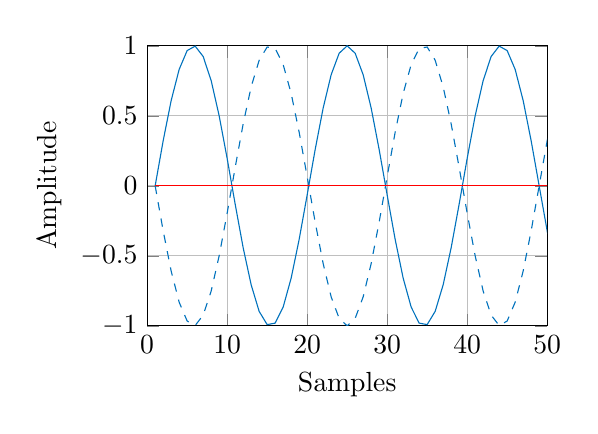
\begin{tikzpicture}

\begin{axis}[%
width=2in,
height=1.4in,
xlabel = {Samples},
ylabel = {Amplitude}, 
scale only axis,
xmin=0,
xmax=50,
xmajorgrids,
ymin=-1,
ymax=1,
ymajorgrids,
axis background/.style={fill=white}
]
\addplot [color=mycolor1,solid,forget plot]
  table[row sep=crcr]{%
1	0\\
2	0.321439465303162\\
3	0.608761429008721\\
4	0.831469612302545\\
5	0.965925826289068\\
6	0.997858923238603\\
7	0.923879532511287\\
8	0.751839807478978\\
9	0.5\\
10	0.195090322016128\\
11	-0.130526192220051\\
12	-0.442288690219001\\
13	-0.707106781186548\\
14	-0.896872741532688\\
15	-0.99144486137381\\
16	-0.98078528040323\\
17	-0.866025403784439\\
18	-0.659345815100069\\
19	-0.38268343236509\\
20	-0.0654031292301428\\
21	0.25881904510252\\
22	0.555570233019602\\
23	0.793353340291235\\
24	0.946930129495105\\
25	1\\
26	0.946930129495106\\
27	0.793353340291235\\
28	0.555570233019604\\
29	0.258819045102523\\
30	-0.0654031292301431\\
31	-0.38268343236509\\
32	-0.659345815100069\\
33	-0.866025403784438\\
34	-0.98078528040323\\
35	-0.991444861373811\\
36	-0.896872741532689\\
37	-0.707106781186547\\
38	-0.442288690219002\\
39	-0.130526192220051\\
40	0.195090322016127\\
41	0.499999999999999\\
42	0.751839807478976\\
43	0.923879532511286\\
44	0.997858923238604\\
45	0.965925826289069\\
46	0.831469612302546\\
47	0.608761429008723\\
48	0.321439465303162\\
49	-1.16403343982657e-15\\
50	-0.321439465303164\\
51	-0.608761429008723\\
52	-0.831469612302545\\
53	-0.965925826289068\\
54	-0.997858923238603\\
55	-0.923879532511286\\
56	-0.751839807478978\\
57	-0.5\\
58	-0.195090322016128\\
59	0.130526192220052\\
60	0.442288690218998\\
61	0.707106781186548\\
62	0.89687274153269\\
63	0.99144486137381\\
64	0.98078528040323\\
65	0.866025403784438\\
66	0.659345815100069\\
67	0.382683432365093\\
68	0.0654031292301461\\
69	-0.258819045102525\\
70	-0.555570233019603\\
71	-0.793353340291236\\
72	-0.946930129495106\\
73	-1\\
74	-0.946930129495105\\
75	-0.793353340291237\\
76	-0.555570233019604\\
77	-0.25881904510252\\
78	0.0654031292301442\\
79	0.382683432365091\\
80	0.65934581510007\\
81	0.866025403784439\\
82	0.98078528040323\\
83	0.991444861373811\\
84	0.896872741532689\\
85	0.707106781186549\\
86	0.442288690219003\\
87	0.13052619222005\\
88	-0.19509032201613\\
89	-0.499999999999999\\
90	-0.751839807478979\\
91	-0.923879532511286\\
92	-0.997858923238603\\
93	-0.965925826289069\\
94	-0.831469612302548\\
95	-0.608761429008722\\
96	-0.321439465303163\\
97	2.32806687965315e-15\\
};
\addplot [color=mycolor1,dashed,forget plot]
  table[row sep=crcr]{%
1	-0\\
2	-0.321439465303162\\
3	-0.608761429008721\\
4	-0.831469612302545\\
5	-0.965925826289068\\
6	-0.997858923238603\\
7	-0.923879532511287\\
8	-0.751839807478978\\
9	-0.5\\
10	-0.195090322016128\\
11	0.130526192220051\\
12	0.442288690219001\\
13	0.707106781186548\\
14	0.896872741532688\\
15	0.99144486137381\\
16	0.98078528040323\\
17	0.866025403784439\\
18	0.659345815100069\\
19	0.38268343236509\\
20	0.0654031292301428\\
21	-0.25881904510252\\
22	-0.555570233019602\\
23	-0.793353340291235\\
24	-0.946930129495105\\
25	-1\\
26	-0.946930129495106\\
27	-0.793353340291235\\
28	-0.555570233019604\\
29	-0.258819045102523\\
30	0.0654031292301431\\
31	0.38268343236509\\
32	0.659345815100069\\
33	0.866025403784438\\
34	0.98078528040323\\
35	0.991444861373811\\
36	0.896872741532689\\
37	0.707106781186547\\
38	0.442288690219002\\
39	0.130526192220051\\
40	-0.195090322016127\\
41	-0.499999999999999\\
42	-0.751839807478976\\
43	-0.923879532511286\\
44	-0.997858923238604\\
45	-0.965925826289069\\
46	-0.831469612302546\\
47	-0.608761429008723\\
48	-0.321439465303162\\
49	1.16403343982657e-15\\
50	0.321439465303164\\
51	0.608761429008723\\
52	0.831469612302545\\
53	0.965925826289068\\
54	0.997858923238603\\
55	0.923879532511286\\
56	0.751839807478978\\
57	0.5\\
58	0.195090322016128\\
59	-0.130526192220052\\
60	-0.442288690218998\\
61	-0.707106781186548\\
62	-0.89687274153269\\
63	-0.99144486137381\\
64	-0.98078528040323\\
65	-0.866025403784438\\
66	-0.659345815100069\\
67	-0.382683432365093\\
68	-0.0654031292301461\\
69	0.258819045102525\\
70	0.555570233019603\\
71	0.793353340291236\\
72	0.946930129495106\\
73	1\\
74	0.946930129495105\\
75	0.793353340291237\\
76	0.555570233019604\\
77	0.25881904510252\\
78	-0.0654031292301442\\
79	-0.382683432365091\\
80	-0.65934581510007\\
81	-0.866025403784439\\
82	-0.98078528040323\\
83	-0.991444861373811\\
84	-0.896872741532689\\
85	-0.707106781186549\\
86	-0.442288690219003\\
87	-0.13052619222005\\
88	0.19509032201613\\
89	0.499999999999999\\
90	0.751839807478979\\
91	0.923879532511286\\
92	0.997858923238603\\
93	0.965925826289069\\
94	0.831469612302548\\
95	0.608761429008722\\
96	0.321439465303163\\
97	-2.32806687965315e-15\\
};
\addplot [color=red,solid,forget plot]
  table[row sep=crcr]{%
1	0\\
2	0\\
3	0\\
4	0\\
5	0\\
6	0\\
7	0\\
8	0\\
9	0\\
10	0\\
11	0\\
12	0\\
13	0\\
14	0\\
15	0\\
16	0\\
17	0\\
18	0\\
19	0\\
20	0\\
21	0\\
22	0\\
23	0\\
24	0\\
25	0\\
26	0\\
27	0\\
28	0\\
29	0\\
30	0\\
31	0\\
32	0\\
33	0\\
34	0\\
35	0\\
36	0\\
37	0\\
38	0\\
39	0\\
40	0\\
41	0\\
42	0\\
43	0\\
44	0\\
45	0\\
46	0\\
47	0\\
48	0\\
49	0\\
50	0\\
51	0\\
52	0\\
53	0\\
54	0\\
55	0\\
56	0\\
57	0\\
58	0\\
59	0\\
60	0\\
61	0\\
62	0\\
63	0\\
64	0\\
65	0\\
66	0\\
67	0\\
68	0\\
69	0\\
70	0\\
71	0\\
72	0\\
73	0\\
74	0\\
75	0\\
76	0\\
77	0\\
78	0\\
79	0\\
80	0\\
81	0\\
82	0\\
83	0\\
84	0\\
85	0\\
86	0\\
87	0\\
88	0\\
89	0\\
90	0\\
91	0\\
92	0\\
93	0\\
94	0\\
95	0\\
96	0\\
97	0\\
};
\end{axis}
\end{tikzpicture}%
	 		%\caption{2500 Hz}
	 	\end{center}
		\end{column}
	\end{columns}
\end{frame}





\begin{frame}{Introduction}{How does ANC work}		
	\begin{itemize}
		\item Feedforward system
		\begin{itemize}
			\item 1: Reference microphone
			\item 2: Headphone loudspeaker
			\item 3: Error mirophone
			\item 4: Digital signal Processor (DSP)
		\end{itemize}
	\end{itemize}
	\begin{center}
	 	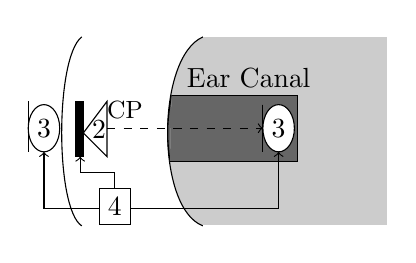
\begin{tikzpicture}
\draw [](-2.22,2.52) node (v1) {} .. controls (-2.56,2.26) and (-2.56,0.34) .. (-2.22,0.12) node (v2) {};

\draw [draw=black,fill=black!20](-0.68,2.52) node (v1) {} .. controls (-1.28,2.26) and (-1.28,0.34) .. (-0.68,0.12) node (v2) {};
\draw [white, fill=black!20](-0.68,2.52) -- (1.66,2.52) -- (1.66,0.12) -- (-0.68,0.12);


\draw [draw=black,fill=black!60](-1.08,1.78) node (v1) {} .. controls (-1.14,1.44) and (-1.14,1.24) .. (-1.1,0.94) node (v2) {};
\draw [draw=black,fill=black!60](-1.08,1.78) -- (0.52,1.78) -- (0.52,0.94) -- (-1.1,0.94);


\draw [draw=black,fill=white] (0.28,1.36) node (v3) {3} ellipse (0.2 and 0.3);
\draw [draw=black,fill=black](0.08,1.66) -- (0.08,1.06);

\draw [draw=black,fill=white] (-2.7,1.36) node (v3) {3} ellipse (0.2 and 0.3);
\draw [draw=black,fill=black](-2.9,1.7) -- (-2.9,1.06);


\draw [draw=black,fill=black] (-2.2,1.7) rectangle (-2.3,1);
\draw (-2.2,1.3) -- (-1.9,1.7) -- (-1.9,1) -- (-2.2,1.3);
\node at (-2,1.34) {2};


\draw[->,dashed] (-1.9,1.36) node[right=6.5,above]{\small{CP}}-- (0.08,1.36);
\draw  (-1.6,0.6) rectangle node{4}(-2,0.14);
\draw [->](-2,0.34) -- (-2.7,0.34) -- (-2.7,1.06);
\draw [->](-1.6,0.34) -- (0.28,0.34) -- (0.28,1.06);
\draw [->](-1.8,0.6) -- (-1.8,0.8) -- (-2.24,0.8) -- (-2.24,1);
\node at (-0.1,2) {Ear Canal};
\end{tikzpicture}
	 	%\caption{2500 Hz}
	\end{center}
\end{frame}




\begin{frame}{Introduction}{Problem of ANC}		
	\begin{columns}
		\begin{column}{0.5\textwidth}
			\begin{itemize}
				\item Counter phase signal delayed 10 samples	
				\begin{itemize}
					\item 250 Hz
					\item 2500 Hz 
				\end{itemize}	
			\end{itemize}
			\vspace{-6.5mm}			
		\begin{center}
	 		% This file was created by matlab2tikz.
%
%The latest updates can be retrieved from
%  http://www.mathworks.com/matlabcentral/fileexchange/22022-matlab2tikz-matlab2tikz
%where you can also make suggestions and rate matlab2tikz.
%
\definecolor{mycolor1}{rgb}{0.00000,0.44700,0.74100}%
%
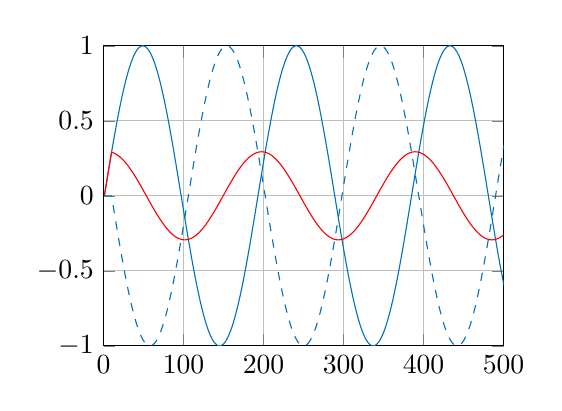
\begin{tikzpicture}

\begin{axis}[%
width=2in,
height=1.5in,
scale only axis,
xmin=0,
xmax=500,
xmajorgrids,
ymin=-1,
ymax=1,
ymajorgrids,
axis background/.style={fill=white}
]
\addplot [color=mycolor1,solid,forget plot]
  table[row sep=crcr]{%
1	0\\
2	0.0327190828217761\\
3	0.0654031292301431\\
4	0.0980171403295606\\
5	0.130526192220052\\
6	0.162895473394589\\
7	0.195090322016128\\
8	0.227076263034373\\
9	0.258819045102521\\
10	0.290284677254462\\
11	0.321439465303162\\
12	0.352250047921233\\
13	0.38268343236509\\
14	0.412707029804395\\
15	0.442288690219001\\
16	0.471396736825998\\
17	0.5\\
18	0.528067850650368\\
19	0.555570233019602\\
20	0.582477696867802\\
21	0.608761429008721\\
22	0.634393284163645\\
23	0.659345815100069\\
24	0.683592302022871\\
25	0.707106781186547\\
26	0.729864072697836\\
27	0.751839807478977\\
28	0.773010453362737\\
29	0.793353340291235\\
30	0.812846684591615\\
31	0.831469612302545\\
32	0.849202181526579\\
33	0.866025403784439\\
34	0.881921264348355\\
35	0.896872741532688\\
36	0.910863824921176\\
37	0.923879532511287\\
38	0.935905926757326\\
39	0.946930129495106\\
40	0.956940335732209\\
41	0.965925826289068\\
42	0.973876979277334\\
43	0.98078528040323\\
44	0.986643332084879\\
45	0.99144486137381\\
46	0.995184726672197\\
47	0.997858923238603\\
48	0.999464587476366\\
49	1\\
50	0.999464587476366\\
51	0.997858923238603\\
52	0.995184726672197\\
53	0.99144486137381\\
54	0.986643332084879\\
55	0.980785280403231\\
56	0.973876979277334\\
57	0.965925826289068\\
58	0.956940335732209\\
59	0.946930129495106\\
60	0.935905926757326\\
61	0.923879532511287\\
62	0.910863824921176\\
63	0.896872741532688\\
64	0.881921264348355\\
65	0.866025403784439\\
66	0.849202181526579\\
67	0.831469612302545\\
68	0.812846684591615\\
69	0.793353340291235\\
70	0.773010453362737\\
71	0.751839807478978\\
72	0.729864072697836\\
73	0.707106781186548\\
74	0.683592302022872\\
75	0.659345815100069\\
76	0.634393284163645\\
77	0.60876142900872\\
78	0.582477696867802\\
79	0.555570233019603\\
80	0.528067850650368\\
81	0.5\\
82	0.471396736825998\\
83	0.442288690219002\\
84	0.412707029804395\\
85	0.38268343236509\\
86	0.352250047921233\\
87	0.321439465303161\\
88	0.290284677254463\\
89	0.258819045102521\\
90	0.227076263034374\\
91	0.195090322016129\\
92	0.162895473394589\\
93	0.130526192220052\\
94	0.0980171403295608\\
95	0.0654031292301431\\
96	0.0327190828217764\\
97	1.22464679914735e-16\\
98	-0.0327190828217758\\
99	-0.0654031292301424\\
100	-0.0980171403295606\\
101	-0.130526192220051\\
102	-0.162895473394588\\
103	-0.195090322016128\\
104	-0.227076263034373\\
105	-0.258819045102521\\
106	-0.290284677254462\\
107	-0.321439465303162\\
108	-0.352250047921233\\
109	-0.382683432365089\\
110	-0.412707029804395\\
111	-0.442288690219001\\
112	-0.471396736825998\\
113	-0.5\\
114	-0.528067850650368\\
115	-0.555570233019602\\
116	-0.582477696867802\\
117	-0.608761429008721\\
118	-0.634393284163645\\
119	-0.659345815100069\\
120	-0.683592302022871\\
121	-0.707106781186548\\
122	-0.729864072697836\\
123	-0.751839807478977\\
124	-0.773010453362737\\
125	-0.793353340291235\\
126	-0.812846684591615\\
127	-0.831469612302545\\
128	-0.849202181526579\\
129	-0.866025403784438\\
130	-0.881921264348354\\
131	-0.896872741532688\\
132	-0.910863824921175\\
133	-0.923879532511287\\
134	-0.935905926757326\\
135	-0.946930129495106\\
136	-0.956940335732209\\
137	-0.965925826289068\\
138	-0.973876979277334\\
139	-0.98078528040323\\
140	-0.986643332084879\\
141	-0.99144486137381\\
142	-0.995184726672197\\
143	-0.997858923238603\\
144	-0.999464587476366\\
145	-1\\
146	-0.999464587476366\\
147	-0.997858923238604\\
148	-0.995184726672197\\
149	-0.99144486137381\\
150	-0.986643332084879\\
151	-0.98078528040323\\
152	-0.973876979277334\\
153	-0.965925826289068\\
154	-0.956940335732209\\
155	-0.946930129495105\\
156	-0.935905926757326\\
157	-0.923879532511287\\
158	-0.910863824921176\\
159	-0.896872741532688\\
160	-0.881921264348355\\
161	-0.866025403784439\\
162	-0.849202181526579\\
163	-0.831469612302545\\
164	-0.812846684591615\\
165	-0.793353340291236\\
166	-0.773010453362737\\
167	-0.751839807478978\\
168	-0.729864072697836\\
169	-0.707106781186548\\
170	-0.683592302022872\\
171	-0.659345815100069\\
172	-0.634393284163646\\
173	-0.60876142900872\\
174	-0.582477696867802\\
175	-0.555570233019603\\
176	-0.528067850650368\\
177	-0.5\\
178	-0.471396736825998\\
179	-0.442288690219002\\
180	-0.412707029804395\\
181	-0.38268343236509\\
182	-0.352250047921234\\
183	-0.321439465303162\\
184	-0.290284677254463\\
185	-0.258819045102522\\
186	-0.227076263034374\\
187	-0.195090322016129\\
188	-0.162895473394589\\
189	-0.130526192220052\\
190	-0.0980171403295605\\
191	-0.0654031292301437\\
192	-0.0327190828217766\\
193	-2.44929359829471e-16\\
194	0.0327190828217752\\
195	0.0654031292301423\\
196	0.0980171403295609\\
197	0.13052619222005\\
198	0.162895473394589\\
199	0.195090322016128\\
200	0.227076263034373\\
201	0.25881904510252\\
202	0.290284677254462\\
203	0.321439465303161\\
204	0.352250047921233\\
205	0.382683432365089\\
206	0.412707029804394\\
207	0.442288690219002\\
208	0.471396736825997\\
209	0.5\\
210	0.528067850650368\\
211	0.555570233019601\\
212	0.582477696867802\\
213	0.608761429008721\\
214	0.634393284163645\\
215	0.659345815100068\\
216	0.683592302022872\\
217	0.707106781186547\\
218	0.729864072697836\\
219	0.751839807478978\\
220	0.773010453362736\\
221	0.793353340291235\\
222	0.812846684591615\\
223	0.831469612302545\\
224	0.849202181526578\\
225	0.866025403784438\\
226	0.881921264348355\\
227	0.896872741532689\\
228	0.910863824921175\\
229	0.923879532511287\\
230	0.935905926757326\\
231	0.946930129495105\\
232	0.956940335732209\\
233	0.965925826289068\\
234	0.973876979277334\\
235	0.98078528040323\\
236	0.986643332084879\\
237	0.99144486137381\\
238	0.995184726672197\\
239	0.997858923238603\\
240	0.999464587476366\\
241	1\\
242	0.999464587476366\\
243	0.997858923238603\\
244	0.995184726672197\\
245	0.99144486137381\\
246	0.986643332084879\\
247	0.98078528040323\\
248	0.973876979277334\\
249	0.965925826289068\\
250	0.956940335732209\\
251	0.946930129495106\\
252	0.935905926757325\\
253	0.923879532511287\\
254	0.910863824921176\\
255	0.896872741532688\\
256	0.881921264348355\\
257	0.866025403784439\\
258	0.849202181526579\\
259	0.831469612302547\\
260	0.812846684591615\\
261	0.793353340291235\\
262	0.773010453362738\\
263	0.751839807478978\\
264	0.729864072697835\\
265	0.707106781186548\\
266	0.683592302022871\\
267	0.65934581510007\\
268	0.634393284163647\\
269	0.608761429008721\\
270	0.582477696867803\\
271	0.555570233019602\\
272	0.528067850650369\\
273	0.5\\
274	0.471396736825998\\
275	0.442288690219001\\
276	0.412707029804396\\
277	0.382683432365091\\
278	0.352250047921233\\
279	0.321439465303162\\
280	0.290284677254463\\
281	0.258819045102523\\
282	0.227076263034374\\
283	0.195090322016128\\
284	0.162895473394589\\
285	0.130526192220053\\
286	0.0980171403295624\\
287	0.0654031292301438\\
288	0.0327190828217758\\
289	3.67394039744206e-16\\
290	-0.0327190828217751\\
291	-0.0654031292301431\\
292	-0.0980171403295617\\
293	-0.13052619222005\\
294	-0.162895473394588\\
295	-0.195090322016126\\
296	-0.227076263034373\\
297	-0.25881904510252\\
298	-0.290284677254461\\
299	-0.32143946530316\\
300	-0.352250047921234\\
301	-0.38268343236509\\
302	-0.412707029804394\\
303	-0.442288690219\\
304	-0.471396736825996\\
305	-0.500000000000001\\
306	-0.528067850650368\\
307	-0.555570233019602\\
308	-0.582477696867801\\
309	-0.608761429008722\\
310	-0.634393284163645\\
311	-0.659345815100069\\
312	-0.68359230202287\\
313	-0.707106781186547\\
314	-0.729864072697835\\
315	-0.751839807478977\\
316	-0.773010453362736\\
317	-0.793353340291235\\
318	-0.812846684591614\\
319	-0.831469612302545\\
320	-0.849202181526578\\
321	-0.866025403784438\\
322	-0.881921264348355\\
323	-0.896872741532689\\
324	-0.910863824921176\\
325	-0.923879532511286\\
326	-0.935905926757325\\
327	-0.946930129495105\\
328	-0.956940335732209\\
329	-0.965925826289068\\
330	-0.973876979277333\\
331	-0.98078528040323\\
332	-0.986643332084879\\
333	-0.99144486137381\\
334	-0.995184726672197\\
335	-0.997858923238603\\
336	-0.999464587476366\\
337	-1\\
338	-0.999464587476366\\
339	-0.997858923238604\\
340	-0.995184726672197\\
341	-0.99144486137381\\
342	-0.986643332084879\\
343	-0.980785280403231\\
344	-0.973876979277334\\
345	-0.965925826289068\\
346	-0.956940335732209\\
347	-0.946930129495106\\
348	-0.935905926757326\\
349	-0.923879532511287\\
350	-0.910863824921176\\
351	-0.896872741532688\\
352	-0.881921264348356\\
353	-0.866025403784439\\
354	-0.849202181526579\\
355	-0.831469612302546\\
356	-0.812846684591616\\
357	-0.793353340291236\\
358	-0.773010453362738\\
359	-0.751839807478977\\
360	-0.729864072697836\\
361	-0.707106781186548\\
362	-0.683592302022871\\
363	-0.65934581510007\\
364	-0.634393284163645\\
365	-0.608761429008721\\
366	-0.582477696867803\\
367	-0.555570233019604\\
368	-0.528067850650367\\
369	-0.500000000000001\\
370	-0.471396736825998\\
371	-0.442288690219002\\
372	-0.412707029804395\\
373	-0.382683432365091\\
374	-0.352250047921235\\
375	-0.321439465303162\\
376	-0.290284677254464\\
377	-0.258819045102521\\
378	-0.227076263034376\\
379	-0.195090322016128\\
380	-0.162895473394591\\
381	-0.130526192220053\\
382	-0.0980171403295608\\
383	-0.0654031292301439\\
384	-0.0327190828217795\\
385	-4.89858719658941e-16\\
386	0.032719082821775\\
387	0.0654031292301412\\
388	0.0980171403295598\\
389	0.13052619222005\\
390	0.162895473394588\\
391	0.195090322016129\\
392	0.227076263034373\\
393	0.258819045102518\\
394	0.290284677254461\\
395	0.321439465303161\\
396	0.352250047921232\\
397	0.38268343236509\\
398	0.412707029804394\\
399	0.442288690219\\
400	0.471396736825999\\
401	0.499999999999999\\
402	0.528067850650366\\
403	0.555570233019602\\
404	0.582477696867802\\
405	0.608761429008719\\
406	0.634393284163646\\
407	0.659345815100068\\
408	0.683592302022871\\
409	0.707106781186547\\
410	0.729864072697835\\
411	0.751839807478977\\
412	0.773010453362735\\
413	0.793353340291236\\
414	0.812846684591614\\
415	0.831469612302544\\
416	0.849202181526578\\
417	0.866025403784439\\
418	0.881921264348354\\
419	0.896872741532688\\
420	0.910863824921175\\
421	0.923879532511286\\
422	0.935905926757326\\
423	0.946930129495105\\
424	0.956940335732208\\
425	0.965925826289068\\
426	0.973876979277333\\
427	0.98078528040323\\
428	0.986643332084879\\
429	0.99144486137381\\
430	0.995184726672197\\
431	0.997858923238604\\
432	0.999464587476366\\
433	1\\
434	0.999464587476366\\
435	0.997858923238603\\
436	0.995184726672197\\
437	0.99144486137381\\
438	0.986643332084879\\
439	0.980785280403231\\
440	0.973876979277334\\
441	0.965925826289069\\
442	0.956940335732209\\
443	0.946930129495106\\
444	0.935905926757326\\
445	0.923879532511287\\
446	0.910863824921177\\
447	0.896872741532689\\
448	0.881921264348356\\
449	0.866025403784439\\
450	0.849202181526579\\
451	0.831469612302546\\
452	0.812846684591617\\
453	0.793353340291234\\
454	0.773010453362738\\
455	0.751839807478979\\
456	0.729864072697836\\
457	0.707106781186549\\
458	0.683592302022873\\
459	0.659345815100068\\
460	0.634393284163647\\
461	0.608761429008723\\
462	0.582477696867802\\
463	0.555570233019603\\
464	0.528067850650369\\
465	0.5\\
466	0.471396736825998\\
467	0.442288690219003\\
468	0.412707029804397\\
469	0.382683432365091\\
470	0.352250047921235\\
471	0.321439465303164\\
472	0.290284677254462\\
473	0.258819045102523\\
474	0.227076263034376\\
475	0.19509032201613\\
476	0.162895473394589\\
477	0.130526192220053\\
478	0.0980171403295609\\
479	0.0654031292301458\\
480	0.0327190828217761\\
481	-1.16403343982657e-15\\
482	-0.0327190828217784\\
483	-0.0654031292301428\\
484	-0.0980171403295579\\
485	-0.130526192220055\\
486	-0.16289547339459\\
487	-0.195090322016127\\
488	-0.227076263034373\\
489	-0.258819045102523\\
490	-0.290284677254461\\
491	-0.321439465303161\\
492	-0.352250047921237\\
493	-0.382683432365091\\
494	-0.412707029804397\\
495	-0.442288690219001\\
496	-0.471396736825999\\
497	-0.499999999999999\\
498	-0.528067850650368\\
499	-0.5555702330196\\
500	-0.582477696867804\\
501	-0.608761429008723\\
502	-0.634393284163646\\
503	-0.65934581510007\\
504	-0.683592302022873\\
505	-0.707106781186548\\
506	-0.729864072697834\\
507	-0.751839807478977\\
508	-0.773010453362737\\
509	-0.793353340291236\\
510	-0.812846684591616\\
511	-0.831469612302547\\
512	-0.849202181526579\\
513	-0.866025403784439\\
514	-0.881921264348355\\
515	-0.896872741532688\\
516	-0.910863824921176\\
517	-0.923879532511286\\
518	-0.935905926757326\\
519	-0.946930129495107\\
520	-0.956940335732209\\
521	-0.965925826289068\\
522	-0.973876979277334\\
523	-0.980785280403231\\
524	-0.986643332084879\\
525	-0.99144486137381\\
526	-0.995184726672197\\
527	-0.997858923238604\\
528	-0.999464587476366\\
529	-1\\
530	-0.999464587476366\\
531	-0.997858923238603\\
532	-0.995184726672197\\
533	-0.991444861373811\\
534	-0.986643332084879\\
535	-0.98078528040323\\
536	-0.973876979277333\\
537	-0.965925826289069\\
538	-0.956940335732208\\
539	-0.946930129495105\\
540	-0.935905926757326\\
541	-0.923879532511287\\
542	-0.910863824921175\\
543	-0.896872741532689\\
544	-0.881921264348355\\
545	-0.866025403784438\\
546	-0.849202181526578\\
547	-0.831469612302544\\
548	-0.812846684591615\\
549	-0.793353340291234\\
550	-0.773010453362736\\
551	-0.751839807478978\\
552	-0.729864072697837\\
553	-0.707106781186546\\
554	-0.683592302022869\\
555	-0.659345815100069\\
556	-0.634393284163644\\
557	-0.608761429008719\\
558	-0.582477696867802\\
559	-0.555570233019604\\
560	-0.528067850650369\\
561	-0.5\\
562	-0.471396736826\\
563	-0.442288690218999\\
564	-0.412707029804392\\
565	-0.382683432365089\\
566	-0.352250047921232\\
567	-0.321439465303162\\
568	-0.290284677254462\\
569	-0.258819045102519\\
570	-0.227076263034374\\
571	-0.195090322016132\\
572	-0.162895473394588\\
573	-0.13052619222005\\
574	-0.098017140329561\\
575	-0.0654031292301424\\
576	-0.0327190828217744\\
577	-7.34788079488412e-16\\
578	0.0327190828217765\\
579	0.0654031292301409\\
580	0.0980171403295595\\
581	0.130526192220055\\
582	0.16289547339459\\
583	0.19509032201613\\
584	0.227076263034376\\
585	0.258819045102521\\
586	0.290284677254461\\
587	0.321439465303164\\
588	0.352250047921234\\
589	0.382683432365088\\
590	0.412707029804397\\
591	0.442288690219005\\
592	0.471396736825999\\
593	0.500000000000002\\
594	0.528067850650368\\
595	0.555570233019603\\
596	0.582477696867804\\
597	0.608761429008717\\
598	0.634393284163646\\
599	0.65934581510007\\
600	0.683592302022871\\
601	0.707106781186548\\
602	0.729864072697836\\
603	0.751839807478977\\
604	0.773010453362737\\
605	0.793353340291236\\
606	0.812846684591614\\
607	0.831469612302545\\
608	0.849202181526579\\
609	0.866025403784439\\
610	0.881921264348356\\
611	0.896872741532688\\
612	0.910863824921175\\
613	0.923879532511286\\
614	0.935905926757326\\
615	0.946930129495105\\
616	0.956940335732208\\
617	0.965925826289069\\
618	0.973876979277334\\
619	0.980785280403231\\
620	0.986643332084879\\
621	0.99144486137381\\
622	0.995184726672197\\
623	0.997858923238603\\
624	0.999464587476366\\
625	1\\
626	0.999464587476366\\
627	0.997858923238604\\
628	0.995184726672197\\
629	0.99144486137381\\
630	0.986643332084879\\
631	0.98078528040323\\
632	0.973876979277334\\
633	0.965925826289069\\
634	0.956940335732209\\
635	0.946930129495105\\
636	0.935905926757325\\
637	0.923879532511286\\
638	0.910863824921176\\
639	0.896872741532689\\
640	0.881921264348354\\
641	0.866025403784438\\
642	0.84920218152658\\
643	0.831469612302546\\
644	0.812846684591613\\
645	0.793353340291235\\
646	0.773010453362736\\
647	0.751839807478978\\
648	0.729864072697835\\
649	0.707106781186546\\
650	0.683592302022872\\
651	0.659345815100069\\
652	0.634393284163644\\
653	0.608761429008721\\
654	0.582477696867802\\
655	0.555570233019601\\
656	0.528067850650369\\
657	0.5\\
658	0.471396736825997\\
659	0.442288690219003\\
660	0.412707029804395\\
661	0.382683432365089\\
662	0.352250047921232\\
663	0.321439465303159\\
664	0.290284677254459\\
665	0.258819045102523\\
666	0.227076263034374\\
667	0.195090322016125\\
668	0.162895473394591\\
669	0.130526192220053\\
670	0.0980171403295611\\
671	0.0654031292301425\\
672	0.0327190828217745\\
673	8.57252759403147e-16\\
674	-0.0327190828217764\\
675	-0.0654031292301444\\
676	-0.0980171403295594\\
677	-0.130526192220048\\
678	-0.16289547339459\\
679	-0.195090322016127\\
680	-0.227076263034373\\
681	-0.258819045102521\\
682	-0.290284677254464\\
683	-0.321439465303161\\
684	-0.352250047921234\\
685	-0.382683432365091\\
686	-0.412707029804394\\
687	-0.442288690219001\\
688	-0.471396736825995\\
689	-0.500000000000002\\
690	-0.528067850650371\\
691	-0.555570233019603\\
692	-0.582477696867801\\
693	-0.608761429008723\\
694	-0.634393284163646\\
695	-0.659345815100067\\
696	-0.68359230202287\\
697	-0.707106781186548\\
698	-0.729864072697836\\
699	-0.751839807478979\\
700	-0.773010453362737\\
701	-0.793353340291236\\
702	-0.812846684591616\\
703	-0.831469612302545\\
704	-0.849202181526579\\
705	-0.866025403784439\\
706	-0.881921264348355\\
707	-0.896872741532688\\
708	-0.910863824921176\\
709	-0.923879532511288\\
710	-0.935905926757326\\
711	-0.946930129495106\\
712	-0.956940335732209\\
713	-0.965925826289068\\
714	-0.973876979277334\\
715	-0.98078528040323\\
716	-0.986643332084879\\
717	-0.991444861373811\\
718	-0.995184726672197\\
719	-0.997858923238603\\
720	-0.999464587476366\\
721	-1\\
722	-0.999464587476366\\
723	-0.997858923238604\\
724	-0.995184726672197\\
725	-0.99144486137381\\
726	-0.986643332084879\\
727	-0.98078528040323\\
728	-0.973876979277333\\
729	-0.965925826289069\\
730	-0.956940335732209\\
731	-0.946930129495105\\
732	-0.935905926757326\\
733	-0.923879532511288\\
734	-0.910863824921176\\
735	-0.896872741532688\\
736	-0.881921264348355\\
737	-0.866025403784438\\
738	-0.849202181526578\\
739	-0.831469612302546\\
740	-0.812846684591615\\
741	-0.793353340291237\\
742	-0.773010453362738\\
743	-0.751839807478975\\
744	-0.729864072697835\\
745	-0.707106781186549\\
746	-0.683592302022869\\
747	-0.659345815100069\\
748	-0.634393284163647\\
749	-0.608761429008722\\
750	-0.582477696867802\\
751	-0.555570233019604\\
752	-0.528067850650366\\
753	-0.499999999999997\\
754	-0.471396736825997\\
755	-0.442288690219\\
756	-0.412707029804392\\
757	-0.382683432365089\\
758	-0.352250047921232\\
759	-0.321439465303159\\
760	-0.290284677254466\\
761	-0.25881904510252\\
762	-0.227076263034368\\
763	-0.195090322016129\\
764	-0.162895473394588\\
765	-0.13052619222005\\
766	-0.0980171403295612\\
767	-0.0654031292301426\\
768	-0.0327190828217746\\
769	-9.79717439317883e-16\\
770	0.0327190828217798\\
771	0.0654031292301478\\
772	0.0980171403295593\\
773	0.130526192220055\\
774	0.162895473394586\\
775	0.195090322016127\\
776	0.227076263034373\\
777	0.258819045102518\\
778	0.29028467725446\\
779	0.321439465303164\\
780	0.352250047921234\\
781	0.382683432365091\\
782	0.412707029804397\\
783	0.442288690219001\\
784	0.471396736825998\\
785	0.500000000000002\\
786	0.528067850650365\\
787	0.5555702330196\\
788	0.582477696867806\\
789	0.60876142900872\\
790	0.634393284163646\\
791	0.65934581510007\\
792	0.68359230202287\\
793	0.707106781186547\\
794	0.729864072697836\\
795	0.751839807478976\\
796	0.773010453362737\\
797	0.793353340291238\\
798	0.812846684591614\\
799	0.831469612302547\\
800	0.849202181526577\\
801	0.866025403784437\\
802	0.881921264348354\\
803	0.896872741532687\\
804	0.910863824921175\\
805	0.923879532511286\\
806	0.935905926757326\\
807	0.946930129495106\\
808	0.956940335732209\\
809	0.965925826289067\\
810	0.973876979277334\\
811	0.980785280403231\\
812	0.986643332084878\\
813	0.99144486137381\\
814	0.995184726672197\\
815	0.997858923238603\\
816	0.999464587476366\\
817	1\\
818	0.999464587476366\\
819	0.997858923238604\\
820	0.995184726672197\\
821	0.991444861373811\\
822	0.986643332084879\\
823	0.98078528040323\\
824	0.973876979277334\\
825	0.965925826289068\\
826	0.956940335732208\\
827	0.946930129495107\\
828	0.935905926757326\\
829	0.923879532511287\\
830	0.910863824921177\\
831	0.896872741532689\\
832	0.881921264348355\\
833	0.866025403784439\\
834	0.849202181526578\\
835	0.831469612302544\\
836	0.812846684591615\\
837	0.793353340291235\\
838	0.773010453362736\\
839	0.75183980747898\\
840	0.729864072697838\\
841	0.707106781186546\\
842	0.683592302022872\\
843	0.659345815100069\\
844	0.634393284163644\\
845	0.608761429008722\\
846	0.582477696867802\\
847	0.555570233019602\\
848	0.528067850650369\\
849	0.5\\
850	0.471396736825997\\
851	0.442288690219003\\
852	0.412707029804392\\
853	0.382683432365086\\
854	0.352250047921236\\
855	0.321439465303163\\
856	0.290284677254462\\
857	0.258819045102523\\
858	0.227076263034375\\
859	0.195090322016129\\
860	0.162895473394588\\
861	0.13052619222005\\
862	0.0980171403295578\\
863	0.0654031292301428\\
864	0.0327190828217748\\
865	-2.45053155956788e-15\\
866	-0.0327190828217726\\
867	-0.0654031292301441\\
868	-0.0980171403295627\\
869	-0.130526192220051\\
870	-0.162895473394589\\
871	-0.19509032201613\\
872	-0.227076263034373\\
873	-0.258819045102521\\
874	-0.290284677254464\\
875	-0.321439465303161\\
876	-0.352250047921234\\
877	-0.382683432365084\\
878	-0.412707029804397\\
879	-0.442288690219004\\
880	-0.471396736825995\\
881	-0.499999999999999\\
882	-0.528067850650367\\
883	-0.5555702330196\\
884	-0.5824776968678\\
885	-0.60876142900872\\
886	-0.634393284163643\\
887	-0.65934581510007\\
888	-0.683592302022873\\
889	-0.707106781186547\\
890	-0.729864072697836\\
891	-0.751839807478979\\
892	-0.773010453362734\\
893	-0.793353340291233\\
894	-0.812846684591616\\
895	-0.831469612302543\\
896	-0.849202181526579\\
897	-0.866025403784439\\
898	-0.881921264348354\\
899	-0.896872741532688\\
900	-0.910863824921176\\
901	-0.923879532511286\\
902	-0.935905926757326\\
903	-0.946930129495106\\
904	-0.956940335732207\\
905	-0.965925826289069\\
906	-0.973876979277335\\
907	-0.98078528040323\\
908	-0.986643332084879\\
909	-0.99144486137381\\
910	-0.995184726672197\\
911	-0.997858923238603\\
912	-0.999464587476366\\
913	-1\\
914	-0.999464587476366\\
915	-0.997858923238603\\
916	-0.995184726672197\\
917	-0.99144486137381\\
918	-0.986643332084879\\
919	-0.980785280403231\\
920	-0.973876979277333\\
921	-0.965925826289068\\
922	-0.95694033573221\\
923	-0.946930129495105\\
924	-0.935905926757325\\
925	-0.923879532511287\\
926	-0.910863824921176\\
927	-0.896872741532688\\
928	-0.881921264348355\\
929	-0.866025403784439\\
930	-0.849202181526582\\
931	-0.831469612302546\\
932	-0.812846684591613\\
933	-0.793353340291237\\
934	-0.773010453362738\\
935	-0.751839807478978\\
936	-0.729864072697838\\
937	-0.707106781186549\\
938	-0.683592302022872\\
939	-0.659345815100072\\
940	-0.634393284163647\\
941	-0.608761429008719\\
942	-0.582477696867802\\
943	-0.555570233019602\\
944	-0.528067850650366\\
945	-0.500000000000004\\
946	-0.471396736826\\
947	-0.442288690219\\
948	-0.412707029804399\\
949	-0.382683432365093\\
950	-0.352250047921232\\
951	-0.321439465303163\\
952	-0.290284677254463\\
953	-0.25881904510252\\
954	-0.227076263034375\\
955	-0.195090322016129\\
956	-0.162895473394592\\
957	-0.130526192220057\\
958	-0.0980171403295615\\
959	-0.0654031292301429\\
960	-0.0327190828217784\\
961	2.32806687965315e-15\\
};
\addplot [color=mycolor1,dashed,forget plot]
  table[row sep=crcr]{%
1	0\\
2	0\\
3	0\\
4	0\\
5	0\\
6	0\\
7	0\\
8	0\\
9	0\\
10	0\\
11	-0.0327190828217761\\
12	-0.0654031292301431\\
13	-0.0980171403295606\\
14	-0.130526192220052\\
15	-0.162895473394589\\
16	-0.195090322016128\\
17	-0.227076263034373\\
18	-0.258819045102521\\
19	-0.290284677254462\\
20	-0.321439465303162\\
21	-0.352250047921233\\
22	-0.38268343236509\\
23	-0.412707029804395\\
24	-0.442288690219001\\
25	-0.471396736825998\\
26	-0.5\\
27	-0.528067850650368\\
28	-0.555570233019602\\
29	-0.582477696867802\\
30	-0.608761429008721\\
31	-0.634393284163645\\
32	-0.659345815100069\\
33	-0.683592302022871\\
34	-0.707106781186547\\
35	-0.729864072697836\\
36	-0.751839807478977\\
37	-0.773010453362737\\
38	-0.793353340291235\\
39	-0.812846684591615\\
40	-0.831469612302545\\
41	-0.849202181526579\\
42	-0.866025403784439\\
43	-0.881921264348355\\
44	-0.896872741532688\\
45	-0.910863824921176\\
46	-0.923879532511287\\
47	-0.935905926757326\\
48	-0.946930129495106\\
49	-0.956940335732209\\
50	-0.965925826289068\\
51	-0.973876979277334\\
52	-0.98078528040323\\
53	-0.986643332084879\\
54	-0.99144486137381\\
55	-0.995184726672197\\
56	-0.997858923238603\\
57	-0.999464587476366\\
58	-1\\
59	-0.999464587476366\\
60	-0.997858923238603\\
61	-0.995184726672197\\
62	-0.99144486137381\\
63	-0.986643332084879\\
64	-0.980785280403231\\
65	-0.973876979277334\\
66	-0.965925826289068\\
67	-0.956940335732209\\
68	-0.946930129495106\\
69	-0.935905926757326\\
70	-0.923879532511287\\
71	-0.910863824921176\\
72	-0.896872741532688\\
73	-0.881921264348355\\
74	-0.866025403784439\\
75	-0.849202181526579\\
76	-0.831469612302545\\
77	-0.812846684591615\\
78	-0.793353340291235\\
79	-0.773010453362737\\
80	-0.751839807478978\\
81	-0.729864072697836\\
82	-0.707106781186548\\
83	-0.683592302022872\\
84	-0.659345815100069\\
85	-0.634393284163645\\
86	-0.60876142900872\\
87	-0.582477696867802\\
88	-0.555570233019603\\
89	-0.528067850650368\\
90	-0.5\\
91	-0.471396736825998\\
92	-0.442288690219002\\
93	-0.412707029804395\\
94	-0.38268343236509\\
95	-0.352250047921233\\
96	-0.321439465303161\\
97	-0.290284677254463\\
98	-0.258819045102521\\
99	-0.227076263034374\\
100	-0.195090322016129\\
101	-0.162895473394589\\
102	-0.130526192220052\\
103	-0.0980171403295608\\
104	-0.0654031292301431\\
105	-0.0327190828217764\\
106	-1.22464679914735e-16\\
107	0.0327190828217758\\
108	0.0654031292301424\\
109	0.0980171403295606\\
110	0.130526192220051\\
111	0.162895473394588\\
112	0.195090322016128\\
113	0.227076263034373\\
114	0.258819045102521\\
115	0.290284677254462\\
116	0.321439465303162\\
117	0.352250047921233\\
118	0.382683432365089\\
119	0.412707029804395\\
120	0.442288690219001\\
121	0.471396736825998\\
122	0.5\\
123	0.528067850650368\\
124	0.555570233019602\\
125	0.582477696867802\\
126	0.608761429008721\\
127	0.634393284163645\\
128	0.659345815100069\\
129	0.683592302022871\\
130	0.707106781186548\\
131	0.729864072697836\\
132	0.751839807478977\\
133	0.773010453362737\\
134	0.793353340291235\\
135	0.812846684591615\\
136	0.831469612302545\\
137	0.849202181526579\\
138	0.866025403784438\\
139	0.881921264348354\\
140	0.896872741532688\\
141	0.910863824921175\\
142	0.923879532511287\\
143	0.935905926757326\\
144	0.946930129495106\\
145	0.956940335732209\\
146	0.965925826289068\\
147	0.973876979277334\\
148	0.98078528040323\\
149	0.986643332084879\\
150	0.99144486137381\\
151	0.995184726672197\\
152	0.997858923238603\\
153	0.999464587476366\\
154	1\\
155	0.999464587476366\\
156	0.997858923238604\\
157	0.995184726672197\\
158	0.99144486137381\\
159	0.986643332084879\\
160	0.98078528040323\\
161	0.973876979277334\\
162	0.965925826289068\\
163	0.956940335732209\\
164	0.946930129495105\\
165	0.935905926757326\\
166	0.923879532511287\\
167	0.910863824921176\\
168	0.896872741532688\\
169	0.881921264348355\\
170	0.866025403784439\\
171	0.849202181526579\\
172	0.831469612302545\\
173	0.812846684591615\\
174	0.793353340291236\\
175	0.773010453362737\\
176	0.751839807478978\\
177	0.729864072697836\\
178	0.707106781186548\\
179	0.683592302022872\\
180	0.659345815100069\\
181	0.634393284163646\\
182	0.60876142900872\\
183	0.582477696867802\\
184	0.555570233019603\\
185	0.528067850650368\\
186	0.5\\
187	0.471396736825998\\
188	0.442288690219002\\
189	0.412707029804395\\
190	0.38268343236509\\
191	0.352250047921234\\
192	0.321439465303162\\
193	0.290284677254463\\
194	0.258819045102522\\
195	0.227076263034374\\
196	0.195090322016129\\
197	0.162895473394589\\
198	0.130526192220052\\
199	0.0980171403295605\\
200	0.0654031292301437\\
201	0.0327190828217766\\
202	2.44929359829471e-16\\
203	-0.0327190828217752\\
204	-0.0654031292301423\\
205	-0.0980171403295609\\
206	-0.13052619222005\\
207	-0.162895473394589\\
208	-0.195090322016128\\
209	-0.227076263034373\\
210	-0.25881904510252\\
211	-0.290284677254462\\
212	-0.321439465303161\\
213	-0.352250047921233\\
214	-0.382683432365089\\
215	-0.412707029804394\\
216	-0.442288690219002\\
217	-0.471396736825997\\
218	-0.5\\
219	-0.528067850650368\\
220	-0.555570233019601\\
221	-0.582477696867802\\
222	-0.608761429008721\\
223	-0.634393284163645\\
224	-0.659345815100068\\
225	-0.683592302022872\\
226	-0.707106781186547\\
227	-0.729864072697836\\
228	-0.751839807478978\\
229	-0.773010453362736\\
230	-0.793353340291235\\
231	-0.812846684591615\\
232	-0.831469612302545\\
233	-0.849202181526578\\
234	-0.866025403784438\\
235	-0.881921264348355\\
236	-0.896872741532689\\
237	-0.910863824921175\\
238	-0.923879532511287\\
239	-0.935905926757326\\
240	-0.946930129495105\\
241	-0.956940335732209\\
242	-0.965925826289068\\
243	-0.973876979277334\\
244	-0.98078528040323\\
245	-0.986643332084879\\
246	-0.99144486137381\\
247	-0.995184726672197\\
248	-0.997858923238603\\
249	-0.999464587476366\\
250	-1\\
251	-0.999464587476366\\
252	-0.997858923238603\\
253	-0.995184726672197\\
254	-0.99144486137381\\
255	-0.986643332084879\\
256	-0.98078528040323\\
257	-0.973876979277334\\
258	-0.965925826289068\\
259	-0.956940335732209\\
260	-0.946930129495106\\
261	-0.935905926757325\\
262	-0.923879532511287\\
263	-0.910863824921176\\
264	-0.896872741532688\\
265	-0.881921264348355\\
266	-0.866025403784439\\
267	-0.849202181526579\\
268	-0.831469612302547\\
269	-0.812846684591615\\
270	-0.793353340291235\\
271	-0.773010453362738\\
272	-0.751839807478978\\
273	-0.729864072697835\\
274	-0.707106781186548\\
275	-0.683592302022871\\
276	-0.65934581510007\\
277	-0.634393284163647\\
278	-0.608761429008721\\
279	-0.582477696867803\\
280	-0.555570233019602\\
281	-0.528067850650369\\
282	-0.5\\
283	-0.471396736825998\\
284	-0.442288690219001\\
285	-0.412707029804396\\
286	-0.382683432365091\\
287	-0.352250047921233\\
288	-0.321439465303162\\
289	-0.290284677254463\\
290	-0.258819045102523\\
291	-0.227076263034374\\
292	-0.195090322016128\\
293	-0.162895473394589\\
294	-0.130526192220053\\
295	-0.0980171403295624\\
296	-0.0654031292301438\\
297	-0.0327190828217758\\
298	-3.67394039744206e-16\\
299	0.0327190828217751\\
300	0.0654031292301431\\
301	0.0980171403295617\\
302	0.13052619222005\\
303	0.162895473394588\\
304	0.195090322016126\\
305	0.227076263034373\\
306	0.25881904510252\\
307	0.290284677254461\\
308	0.32143946530316\\
309	0.352250047921234\\
310	0.38268343236509\\
311	0.412707029804394\\
312	0.442288690219\\
313	0.471396736825996\\
314	0.500000000000001\\
315	0.528067850650368\\
316	0.555570233019602\\
317	0.582477696867801\\
318	0.608761429008722\\
319	0.634393284163645\\
320	0.659345815100069\\
321	0.68359230202287\\
322	0.707106781186547\\
323	0.729864072697835\\
324	0.751839807478977\\
325	0.773010453362736\\
326	0.793353340291235\\
327	0.812846684591614\\
328	0.831469612302545\\
329	0.849202181526578\\
330	0.866025403784438\\
331	0.881921264348355\\
332	0.896872741532689\\
333	0.910863824921176\\
334	0.923879532511286\\
335	0.935905926757325\\
336	0.946930129495105\\
337	0.956940335732209\\
338	0.965925826289068\\
339	0.973876979277333\\
340	0.98078528040323\\
341	0.986643332084879\\
342	0.99144486137381\\
343	0.995184726672197\\
344	0.997858923238603\\
345	0.999464587476366\\
346	1\\
347	0.999464587476366\\
348	0.997858923238604\\
349	0.995184726672197\\
350	0.99144486137381\\
351	0.986643332084879\\
352	0.980785280403231\\
353	0.973876979277334\\
354	0.965925826289068\\
355	0.956940335732209\\
356	0.946930129495106\\
357	0.935905926757326\\
358	0.923879532511287\\
359	0.910863824921176\\
360	0.896872741532688\\
361	0.881921264348356\\
362	0.866025403784439\\
363	0.849202181526579\\
364	0.831469612302546\\
365	0.812846684591616\\
366	0.793353340291236\\
367	0.773010453362738\\
368	0.751839807478977\\
369	0.729864072697836\\
370	0.707106781186548\\
371	0.683592302022871\\
372	0.65934581510007\\
373	0.634393284163645\\
374	0.608761429008721\\
375	0.582477696867803\\
376	0.555570233019604\\
377	0.528067850650367\\
378	0.500000000000001\\
379	0.471396736825998\\
380	0.442288690219002\\
381	0.412707029804395\\
382	0.382683432365091\\
383	0.352250047921235\\
384	0.321439465303162\\
385	0.290284677254464\\
386	0.258819045102521\\
387	0.227076263034376\\
388	0.195090322016128\\
389	0.162895473394591\\
390	0.130526192220053\\
391	0.0980171403295608\\
392	0.0654031292301439\\
393	0.0327190828217795\\
394	4.89858719658941e-16\\
395	-0.032719082821775\\
396	-0.0654031292301412\\
397	-0.0980171403295598\\
398	-0.13052619222005\\
399	-0.162895473394588\\
400	-0.195090322016129\\
401	-0.227076263034373\\
402	-0.258819045102518\\
403	-0.290284677254461\\
404	-0.321439465303161\\
405	-0.352250047921232\\
406	-0.38268343236509\\
407	-0.412707029804394\\
408	-0.442288690219\\
409	-0.471396736825999\\
410	-0.499999999999999\\
411	-0.528067850650366\\
412	-0.555570233019602\\
413	-0.582477696867802\\
414	-0.608761429008719\\
415	-0.634393284163646\\
416	-0.659345815100068\\
417	-0.683592302022871\\
418	-0.707106781186547\\
419	-0.729864072697835\\
420	-0.751839807478977\\
421	-0.773010453362735\\
422	-0.793353340291236\\
423	-0.812846684591614\\
424	-0.831469612302544\\
425	-0.849202181526578\\
426	-0.866025403784439\\
427	-0.881921264348354\\
428	-0.896872741532688\\
429	-0.910863824921175\\
430	-0.923879532511286\\
431	-0.935905926757326\\
432	-0.946930129495105\\
433	-0.956940335732208\\
434	-0.965925826289068\\
435	-0.973876979277333\\
436	-0.98078528040323\\
437	-0.986643332084879\\
438	-0.99144486137381\\
439	-0.995184726672197\\
440	-0.997858923238604\\
441	-0.999464587476366\\
442	-1\\
443	-0.999464587476366\\
444	-0.997858923238603\\
445	-0.995184726672197\\
446	-0.99144486137381\\
447	-0.986643332084879\\
448	-0.980785280403231\\
449	-0.973876979277334\\
450	-0.965925826289069\\
451	-0.956940335732209\\
452	-0.946930129495106\\
453	-0.935905926757326\\
454	-0.923879532511287\\
455	-0.910863824921177\\
456	-0.896872741532689\\
457	-0.881921264348356\\
458	-0.866025403784439\\
459	-0.849202181526579\\
460	-0.831469612302546\\
461	-0.812846684591617\\
462	-0.793353340291234\\
463	-0.773010453362738\\
464	-0.751839807478979\\
465	-0.729864072697836\\
466	-0.707106781186549\\
467	-0.683592302022873\\
468	-0.659345815100068\\
469	-0.634393284163647\\
470	-0.608761429008723\\
471	-0.582477696867802\\
472	-0.555570233019603\\
473	-0.528067850650369\\
474	-0.5\\
475	-0.471396736825998\\
476	-0.442288690219003\\
477	-0.412707029804397\\
478	-0.382683432365091\\
479	-0.352250047921235\\
480	-0.321439465303164\\
481	-0.290284677254462\\
482	-0.258819045102523\\
483	-0.227076263034376\\
484	-0.19509032201613\\
485	-0.162895473394589\\
486	-0.130526192220053\\
487	-0.0980171403295609\\
488	-0.0654031292301458\\
489	-0.0327190828217761\\
490	1.16403343982657e-15\\
491	0.0327190828217784\\
492	0.0654031292301428\\
493	0.0980171403295579\\
494	0.130526192220055\\
495	0.16289547339459\\
496	0.195090322016127\\
497	0.227076263034373\\
498	0.258819045102523\\
499	0.290284677254461\\
500	0.321439465303161\\
501	0.352250047921237\\
502	0.382683432365091\\
503	0.412707029804397\\
504	0.442288690219001\\
505	0.471396736825999\\
506	0.499999999999999\\
507	0.528067850650368\\
508	0.5555702330196\\
509	0.582477696867804\\
510	0.608761429008723\\
511	0.634393284163646\\
512	0.65934581510007\\
513	0.683592302022873\\
514	0.707106781186548\\
515	0.729864072697834\\
516	0.751839807478977\\
517	0.773010453362737\\
518	0.793353340291236\\
519	0.812846684591616\\
520	0.831469612302547\\
521	0.849202181526579\\
522	0.866025403784439\\
523	0.881921264348355\\
524	0.896872741532688\\
525	0.910863824921176\\
526	0.923879532511286\\
527	0.935905926757326\\
528	0.946930129495107\\
529	0.956940335732209\\
530	0.965925826289068\\
531	0.973876979277334\\
532	0.980785280403231\\
533	0.986643332084879\\
534	0.99144486137381\\
535	0.995184726672197\\
536	0.997858923238604\\
537	0.999464587476366\\
538	1\\
539	0.999464587476366\\
540	0.997858923238603\\
541	0.995184726672197\\
542	0.991444861373811\\
543	0.986643332084879\\
544	0.98078528040323\\
545	0.973876979277333\\
546	0.965925826289069\\
547	0.956940335732208\\
548	0.946930129495105\\
549	0.935905926757326\\
550	0.923879532511287\\
551	0.910863824921175\\
552	0.896872741532689\\
553	0.881921264348355\\
554	0.866025403784438\\
555	0.849202181526578\\
556	0.831469612302544\\
557	0.812846684591615\\
558	0.793353340291234\\
559	0.773010453362736\\
560	0.751839807478978\\
561	0.729864072697837\\
562	0.707106781186546\\
563	0.683592302022869\\
564	0.659345815100069\\
565	0.634393284163644\\
566	0.608761429008719\\
567	0.582477696867802\\
568	0.555570233019604\\
569	0.528067850650369\\
570	0.5\\
571	0.471396736826\\
572	0.442288690218999\\
573	0.412707029804392\\
574	0.382683432365089\\
575	0.352250047921232\\
576	0.321439465303162\\
577	0.290284677254462\\
578	0.258819045102519\\
579	0.227076263034374\\
580	0.195090322016132\\
581	0.162895473394588\\
582	0.13052619222005\\
583	0.098017140329561\\
584	0.0654031292301424\\
585	0.0327190828217744\\
586	7.34788079488412e-16\\
587	-0.0327190828217765\\
588	-0.0654031292301409\\
589	-0.0980171403295595\\
590	-0.130526192220055\\
591	-0.16289547339459\\
592	-0.19509032201613\\
593	-0.227076263034376\\
594	-0.258819045102521\\
595	-0.290284677254461\\
596	-0.321439465303164\\
597	-0.352250047921234\\
598	-0.382683432365088\\
599	-0.412707029804397\\
600	-0.442288690219005\\
601	-0.471396736825999\\
602	-0.500000000000002\\
603	-0.528067850650368\\
604	-0.555570233019603\\
605	-0.582477696867804\\
606	-0.608761429008717\\
607	-0.634393284163646\\
608	-0.65934581510007\\
609	-0.683592302022871\\
610	-0.707106781186548\\
611	-0.729864072697836\\
612	-0.751839807478977\\
613	-0.773010453362737\\
614	-0.793353340291236\\
615	-0.812846684591614\\
616	-0.831469612302545\\
617	-0.849202181526579\\
618	-0.866025403784439\\
619	-0.881921264348356\\
620	-0.896872741532688\\
621	-0.910863824921175\\
622	-0.923879532511286\\
623	-0.935905926757326\\
624	-0.946930129495105\\
625	-0.956940335732208\\
626	-0.965925826289069\\
627	-0.973876979277334\\
628	-0.980785280403231\\
629	-0.986643332084879\\
630	-0.99144486137381\\
631	-0.995184726672197\\
632	-0.997858923238603\\
633	-0.999464587476366\\
634	-1\\
635	-0.999464587476366\\
636	-0.997858923238604\\
637	-0.995184726672197\\
638	-0.99144486137381\\
639	-0.986643332084879\\
640	-0.98078528040323\\
641	-0.973876979277334\\
642	-0.965925826289069\\
643	-0.956940335732209\\
644	-0.946930129495105\\
645	-0.935905926757325\\
646	-0.923879532511286\\
647	-0.910863824921176\\
648	-0.896872741532689\\
649	-0.881921264348354\\
650	-0.866025403784438\\
651	-0.84920218152658\\
652	-0.831469612302546\\
653	-0.812846684591613\\
654	-0.793353340291235\\
655	-0.773010453362736\\
656	-0.751839807478978\\
657	-0.729864072697835\\
658	-0.707106781186546\\
659	-0.683592302022872\\
660	-0.659345815100069\\
661	-0.634393284163644\\
662	-0.608761429008721\\
663	-0.582477696867802\\
664	-0.555570233019601\\
665	-0.528067850650369\\
666	-0.5\\
667	-0.471396736825997\\
668	-0.442288690219003\\
669	-0.412707029804395\\
670	-0.382683432365089\\
671	-0.352250047921232\\
672	-0.321439465303159\\
673	-0.290284677254459\\
674	-0.258819045102523\\
675	-0.227076263034374\\
676	-0.195090322016125\\
677	-0.162895473394591\\
678	-0.130526192220053\\
679	-0.0980171403295611\\
680	-0.0654031292301425\\
681	-0.0327190828217745\\
682	-8.57252759403147e-16\\
683	0.0327190828217764\\
684	0.0654031292301444\\
685	0.0980171403295594\\
686	0.130526192220048\\
687	0.16289547339459\\
688	0.195090322016127\\
689	0.227076263034373\\
690	0.258819045102521\\
691	0.290284677254464\\
692	0.321439465303161\\
693	0.352250047921234\\
694	0.382683432365091\\
695	0.412707029804394\\
696	0.442288690219001\\
697	0.471396736825995\\
698	0.500000000000002\\
699	0.528067850650371\\
700	0.555570233019603\\
701	0.582477696867801\\
702	0.608761429008723\\
703	0.634393284163646\\
704	0.659345815100067\\
705	0.68359230202287\\
706	0.707106781186548\\
707	0.729864072697836\\
708	0.751839807478979\\
709	0.773010453362737\\
710	0.793353340291236\\
711	0.812846684591616\\
712	0.831469612302545\\
713	0.849202181526579\\
714	0.866025403784439\\
715	0.881921264348355\\
716	0.896872741532688\\
717	0.910863824921176\\
718	0.923879532511288\\
719	0.935905926757326\\
720	0.946930129495106\\
721	0.956940335732209\\
722	0.965925826289068\\
723	0.973876979277334\\
724	0.98078528040323\\
725	0.986643332084879\\
726	0.991444861373811\\
727	0.995184726672197\\
728	0.997858923238603\\
729	0.999464587476366\\
730	1\\
731	0.999464587476366\\
732	0.997858923238604\\
733	0.995184726672197\\
734	0.99144486137381\\
735	0.986643332084879\\
736	0.98078528040323\\
737	0.973876979277333\\
738	0.965925826289069\\
739	0.956940335732209\\
740	0.946930129495105\\
741	0.935905926757326\\
742	0.923879532511288\\
743	0.910863824921176\\
744	0.896872741532688\\
745	0.881921264348355\\
746	0.866025403784438\\
747	0.849202181526578\\
748	0.831469612302546\\
749	0.812846684591615\\
750	0.793353340291237\\
751	0.773010453362738\\
752	0.751839807478975\\
753	0.729864072697835\\
754	0.707106781186549\\
755	0.683592302022869\\
756	0.659345815100069\\
757	0.634393284163647\\
758	0.608761429008722\\
759	0.582477696867802\\
760	0.555570233019604\\
761	0.528067850650366\\
762	0.499999999999997\\
763	0.471396736825997\\
764	0.442288690219\\
765	0.412707029804392\\
766	0.382683432365089\\
767	0.352250047921232\\
768	0.321439465303159\\
769	0.290284677254466\\
770	0.25881904510252\\
771	0.227076263034368\\
772	0.195090322016129\\
773	0.162895473394588\\
774	0.13052619222005\\
775	0.0980171403295612\\
776	0.0654031292301426\\
777	0.0327190828217746\\
778	9.79717439317883e-16\\
779	-0.0327190828217798\\
780	-0.0654031292301478\\
781	-0.0980171403295593\\
782	-0.130526192220055\\
783	-0.162895473394586\\
784	-0.195090322016127\\
785	-0.227076263034373\\
786	-0.258819045102518\\
787	-0.29028467725446\\
788	-0.321439465303164\\
789	-0.352250047921234\\
790	-0.382683432365091\\
791	-0.412707029804397\\
792	-0.442288690219001\\
793	-0.471396736825998\\
794	-0.500000000000002\\
795	-0.528067850650365\\
796	-0.5555702330196\\
797	-0.582477696867806\\
798	-0.60876142900872\\
799	-0.634393284163646\\
800	-0.65934581510007\\
801	-0.68359230202287\\
802	-0.707106781186547\\
803	-0.729864072697836\\
804	-0.751839807478976\\
805	-0.773010453362737\\
806	-0.793353340291238\\
807	-0.812846684591614\\
808	-0.831469612302547\\
809	-0.849202181526577\\
810	-0.866025403784437\\
811	-0.881921264348354\\
812	-0.896872741532687\\
813	-0.910863824921175\\
814	-0.923879532511286\\
815	-0.935905926757326\\
816	-0.946930129495106\\
817	-0.956940335732209\\
818	-0.965925826289067\\
819	-0.973876979277334\\
820	-0.980785280403231\\
821	-0.986643332084878\\
822	-0.99144486137381\\
823	-0.995184726672197\\
824	-0.997858923238603\\
825	-0.999464587476366\\
826	-1\\
827	-0.999464587476366\\
828	-0.997858923238604\\
829	-0.995184726672197\\
830	-0.991444861373811\\
831	-0.986643332084879\\
832	-0.98078528040323\\
833	-0.973876979277334\\
834	-0.965925826289068\\
835	-0.956940335732208\\
836	-0.946930129495107\\
837	-0.935905926757326\\
838	-0.923879532511287\\
839	-0.910863824921177\\
840	-0.896872741532689\\
841	-0.881921264348355\\
842	-0.866025403784439\\
843	-0.849202181526578\\
844	-0.831469612302544\\
845	-0.812846684591615\\
846	-0.793353340291235\\
847	-0.773010453362736\\
848	-0.75183980747898\\
849	-0.729864072697838\\
850	-0.707106781186546\\
851	-0.683592302022872\\
852	-0.659345815100069\\
853	-0.634393284163644\\
854	-0.608761429008722\\
855	-0.582477696867802\\
856	-0.555570233019602\\
857	-0.528067850650369\\
858	-0.5\\
859	-0.471396736825997\\
860	-0.442288690219003\\
861	-0.412707029804392\\
862	-0.382683432365086\\
863	-0.352250047921236\\
864	-0.321439465303163\\
865	-0.290284677254462\\
866	-0.258819045102523\\
867	-0.227076263034375\\
868	-0.195090322016129\\
869	-0.162895473394588\\
870	-0.13052619222005\\
871	-0.0980171403295578\\
872	-0.0654031292301428\\
873	-0.0327190828217748\\
874	2.45053155956788e-15\\
875	0.0327190828217726\\
876	0.0654031292301441\\
877	0.0980171403295627\\
878	0.130526192220051\\
879	0.162895473394589\\
880	0.19509032201613\\
881	0.227076263034373\\
882	0.258819045102521\\
883	0.290284677254464\\
884	0.321439465303161\\
885	0.352250047921234\\
886	0.382683432365084\\
887	0.412707029804397\\
888	0.442288690219004\\
889	0.471396736825995\\
890	0.499999999999999\\
891	0.528067850650367\\
892	0.5555702330196\\
893	0.5824776968678\\
894	0.60876142900872\\
895	0.634393284163643\\
896	0.65934581510007\\
897	0.683592302022873\\
898	0.707106781186547\\
899	0.729864072697836\\
900	0.751839807478979\\
901	0.773010453362734\\
902	0.793353340291233\\
903	0.812846684591616\\
904	0.831469612302543\\
905	0.849202181526579\\
906	0.866025403784439\\
907	0.881921264348354\\
908	0.896872741532688\\
909	0.910863824921176\\
910	0.923879532511286\\
911	0.935905926757326\\
912	0.946930129495106\\
913	0.956940335732207\\
914	0.965925826289069\\
915	0.973876979277335\\
916	0.98078528040323\\
917	0.986643332084879\\
918	0.99144486137381\\
919	0.995184726672197\\
920	0.997858923238603\\
921	0.999464587476366\\
922	1\\
923	0.999464587476366\\
924	0.997858923238603\\
925	0.995184726672197\\
926	0.99144486137381\\
927	0.986643332084879\\
928	0.980785280403231\\
929	0.973876979277333\\
930	0.965925826289068\\
931	0.95694033573221\\
932	0.946930129495105\\
933	0.935905926757325\\
934	0.923879532511287\\
935	0.910863824921176\\
936	0.896872741532688\\
937	0.881921264348355\\
938	0.866025403784439\\
939	0.849202181526582\\
940	0.831469612302546\\
941	0.812846684591613\\
942	0.793353340291237\\
943	0.773010453362738\\
944	0.751839807478978\\
945	0.729864072697838\\
946	0.707106781186549\\
947	0.683592302022872\\
948	0.659345815100072\\
949	0.634393284163647\\
950	0.608761429008719\\
951	0.582477696867802\\
952	0.555570233019602\\
953	0.528067850650366\\
954	0.500000000000004\\
955	0.471396736826\\
956	0.442288690219\\
957	0.412707029804399\\
958	0.382683432365093\\
959	0.352250047921232\\
960	0.321439465303163\\
961	0.290284677254463\\
962	0.25881904510252\\
963	0.227076263034375\\
964	0.195090322016129\\
965	0.162895473394592\\
966	0.130526192220057\\
967	0.0980171403295615\\
968	0.0654031292301429\\
969	0.0327190828217784\\
970	-2.32806687965315e-15\\
};
\addplot [color=red,solid,forget plot]
  table[row sep=crcr]{%
1	0\\
2	0.0327190828217761\\
3	0.0654031292301431\\
4	0.0980171403295606\\
5	0.130526192220052\\
6	0.162895473394589\\
7	0.195090322016128\\
8	0.227076263034373\\
9	0.258819045102521\\
10	0.290284677254462\\
11	0.288720382481385\\
12	0.28684691869109\\
13	0.284666292035529\\
14	0.282180837584343\\
15	0.279393216824413\\
16	0.276306414809869\\
17	0.272923736965627\\
18	0.269248805547847\\
19	0.26528555576514\\
20	0.261038231564641\\
21	0.256511381087487\\
22	0.251709851798556\\
23	0.246638785295674\\
24	0.24130361180387\\
25	0.23571004436055\\
26	0.229864072697836\\
27	0.223771956828609\\
28	0.217440220343135\\
29	0.210875643423433\\
30	0.204085255582895\\
31	0.1970763281389\\
32	0.18985636642651\\
33	0.182433101761567\\
34	0.174814483161807\\
35	0.167008668834853\\
36	0.159024017442198\\
37	0.15086907914855\\
38	0.14255258646609\\
39	0.13408344490349\\
40	0.125470723429664\\
41	0.116723644762489\\
42	0.107851575492895\\
43	0.0988640160548755\\
44	0.0897705905521906\\
45	0.0805810364526347\\
46	0.0713051941609101\\
47	0.0619529964812778\\
48	0.05253445798126\\
49	0.0430596642677912\\
50	0.0335387611872975\\
51	0.0239819439612698\\
52	0.0143994462689665\\
53	0.00480152928893141\\
54	-0.00480152928893141\\
55	-0.0143994462689663\\
56	-0.0239819439612698\\
57	-0.0335387611872974\\
58	-0.0430596642677911\\
59	-0.05253445798126\\
60	-0.0619529964812777\\
61	-0.0713051941609102\\
62	-0.0805810364526345\\
63	-0.0897705905521906\\
64	-0.0988640160548753\\
65	-0.107851575492895\\
66	-0.116723644762489\\
67	-0.125470723429664\\
68	-0.13408344490349\\
69	-0.142552586466091\\
70	-0.15086907914855\\
71	-0.159024017442198\\
72	-0.167008668834853\\
73	-0.174814483161808\\
74	-0.182433101761567\\
75	-0.18985636642651\\
76	-0.1970763281389\\
77	-0.204085255582895\\
78	-0.210875643423433\\
79	-0.217440220343135\\
80	-0.22377195682861\\
81	-0.229864072697835\\
82	-0.23571004436055\\
83	-0.24130361180387\\
84	-0.246638785295674\\
85	-0.251709851798556\\
86	-0.256511381087487\\
87	-0.261038231564641\\
88	-0.26528555576514\\
89	-0.269248805547847\\
90	-0.272923736965627\\
91	-0.276306414809869\\
92	-0.279393216824413\\
93	-0.282180837584343\\
94	-0.284666292035529\\
95	-0.28684691869109\\
96	-0.288720382481385\\
97	-0.290284677254463\\
98	-0.291538127924297\\
99	-0.292479392264516\\
100	-0.293107462345689\\
101	-0.29342166561464\\
102	-0.29342166561464\\
103	-0.293107462345689\\
104	-0.292479392264517\\
105	-0.291538127924297\\
106	-0.290284677254462\\
107	-0.288720382481386\\
108	-0.286846918691091\\
109	-0.284666292035529\\
110	-0.282180837584343\\
111	-0.279393216824413\\
112	-0.27630641480987\\
113	-0.272923736965626\\
114	-0.269248805547848\\
115	-0.26528555576514\\
116	-0.26103823156464\\
117	-0.256511381087487\\
118	-0.251709851798556\\
119	-0.246638785295674\\
120	-0.24130361180387\\
121	-0.23571004436055\\
122	-0.229864072697836\\
123	-0.223771956828609\\
124	-0.217440220343135\\
125	-0.210875643423433\\
126	-0.204085255582894\\
127	-0.1970763281389\\
128	-0.18985636642651\\
129	-0.182433101761567\\
130	-0.174814483161807\\
131	-0.167008668834853\\
132	-0.159024017442198\\
133	-0.150869079148549\\
134	-0.142552586466091\\
135	-0.13408344490349\\
136	-0.125470723429664\\
137	-0.116723644762489\\
138	-0.107851575492895\\
139	-0.0988640160548758\\
140	-0.0897705905521907\\
141	-0.0805810364526348\\
142	-0.0713051941609104\\
143	-0.0619529964812779\\
144	-0.0525344579812601\\
145	-0.0430596642677912\\
146	-0.0335387611872974\\
147	-0.0239819439612698\\
148	-0.0143994462689667\\
149	-0.00480152928893152\\
150	0.00480152928893107\\
151	0.0143994462689665\\
152	0.0239819439612696\\
153	0.0335387611872975\\
154	0.0430596642677911\\
155	0.0525344579812602\\
156	0.0619529964812779\\
157	0.0713051941609101\\
158	0.0805810364526345\\
159	0.0897705905521907\\
160	0.0988640160548754\\
161	0.107851575492895\\
162	0.116723644762489\\
163	0.125470723429663\\
164	0.13408344490349\\
165	0.14255258646609\\
166	0.15086907914855\\
167	0.159024017442198\\
168	0.167008668834852\\
169	0.174814483161807\\
170	0.182433101761567\\
171	0.18985636642651\\
172	0.1970763281389\\
173	0.204085255582895\\
174	0.210875643423433\\
175	0.217440220343134\\
176	0.22377195682861\\
177	0.229864072697836\\
178	0.23571004436055\\
179	0.24130361180387\\
180	0.246638785295674\\
181	0.251709851798556\\
182	0.256511381087486\\
183	0.26103823156464\\
184	0.26528555576514\\
185	0.269248805547846\\
186	0.272923736965627\\
187	0.276306414809869\\
188	0.279393216824413\\
189	0.282180837584343\\
190	0.28466629203553\\
191	0.28684691869109\\
192	0.288720382481385\\
193	0.290284677254463\\
194	0.291538127924297\\
195	0.292479392264516\\
196	0.29310746234569\\
197	0.293421665614639\\
198	0.29342166561464\\
199	0.293107462345689\\
200	0.292479392264516\\
201	0.291538127924297\\
202	0.290284677254462\\
203	0.288720382481385\\
204	0.28684691869109\\
205	0.284666292035528\\
206	0.282180837584344\\
207	0.279393216824413\\
208	0.276306414809869\\
209	0.272923736965627\\
210	0.269248805547848\\
211	0.265285555765139\\
212	0.261038231564641\\
213	0.256511381087488\\
214	0.251709851798556\\
215	0.246638785295674\\
216	0.24130361180387\\
217	0.23571004436055\\
218	0.229864072697836\\
219	0.223771956828609\\
220	0.217440220343135\\
221	0.210875643423433\\
222	0.204085255582894\\
223	0.1970763281389\\
224	0.18985636642651\\
225	0.182433101761567\\
226	0.174814483161808\\
227	0.167008668834853\\
228	0.159024017442198\\
229	0.150869079148551\\
230	0.142552586466091\\
231	0.134083444903491\\
232	0.125470723429664\\
233	0.11672364476249\\
234	0.107851575492895\\
235	0.0988640160548755\\
236	0.0897705905521902\\
237	0.0805810364526348\\
238	0.0713051941609103\\
239	0.0619529964812776\\
240	0.0525344579812603\\
241	0.0430596642677912\\
242	0.0335387611872974\\
243	0.02398194396127\\
244	0.0143994462689666\\
245	0.00480152928893174\\
246	-0.00480152928893118\\
247	-0.0143994462689665\\
248	-0.0239819439612698\\
249	-0.0335387611872972\\
250	-0.0430596642677907\\
251	-0.0525344579812599\\
252	-0.0619529964812781\\
253	-0.0713051941609095\\
254	-0.0805810364526345\\
255	-0.0897705905521909\\
256	-0.0988640160548752\\
257	-0.107851575492894\\
258	-0.11672364476249\\
259	-0.125470723429663\\
260	-0.134083444903491\\
261	-0.14255258646609\\
262	-0.15086907914855\\
263	-0.159024017442198\\
264	-0.167008668834853\\
265	-0.174814483161807\\
266	-0.182433101761568\\
267	-0.189856366426509\\
268	-0.1970763281389\\
269	-0.204085255582894\\
270	-0.210875643423432\\
271	-0.217440220343135\\
272	-0.22377195682861\\
273	-0.229864072697835\\
274	-0.23571004436055\\
275	-0.241303611803871\\
276	-0.246638785295673\\
277	-0.251709851798556\\
278	-0.256511381087488\\
279	-0.261038231564641\\
280	-0.265285555765139\\
281	-0.269248805547846\\
282	-0.272923736965626\\
283	-0.27630641480987\\
284	-0.279393216824412\\
285	-0.282180837584344\\
286	-0.284666292035528\\
287	-0.286846918691089\\
288	-0.288720382481386\\
289	-0.290284677254463\\
290	-0.291538127924298\\
291	-0.292479392264517\\
292	-0.29310746234569\\
293	-0.293421665614639\\
294	-0.293421665614641\\
295	-0.293107462345688\\
296	-0.292479392264517\\
297	-0.291538127924296\\
298	-0.290284677254461\\
299	-0.288720382481385\\
300	-0.286846918691091\\
301	-0.284666292035528\\
302	-0.282180837584344\\
303	-0.279393216824412\\
304	-0.27630641480987\\
305	-0.272923736965627\\
306	-0.269248805547848\\
307	-0.265285555765141\\
308	-0.261038231564641\\
309	-0.256511381087488\\
310	-0.251709851798555\\
311	-0.246638785295675\\
312	-0.24130361180387\\
313	-0.235710044360551\\
314	-0.229864072697835\\
315	-0.223771956828609\\
316	-0.217440220343134\\
317	-0.210875643423434\\
318	-0.204085255582893\\
319	-0.1970763281389\\
320	-0.189856366426509\\
321	-0.182433101761568\\
322	-0.174814483161808\\
323	-0.167008668834853\\
324	-0.159024017442199\\
325	-0.150869079148551\\
326	-0.14255258646609\\
327	-0.134083444903491\\
328	-0.125470723429664\\
329	-0.116723644762489\\
330	-0.107851575492896\\
331	-0.0988640160548754\\
332	-0.0897705905521904\\
333	-0.0805810364526345\\
334	-0.0713051941609105\\
335	-0.0619529964812783\\
336	-0.0525344579812602\\
337	-0.043059664267791\\
338	-0.0335387611872979\\
339	-0.0239819439612702\\
340	-0.0143994462689669\\
341	-0.00480152928893141\\
342	0.00480152928893118\\
343	0.0143994462689663\\
344	0.0239819439612693\\
345	0.0335387611872977\\
346	0.0430596642677907\\
347	0.0525344579812599\\
348	0.0619529964812775\\
349	0.0713051941609097\\
350	0.0805810364526343\\
351	0.0897705905521909\\
352	0.0988640160548746\\
353	0.107851575492895\\
354	0.116723644762489\\
355	0.125470723429664\\
356	0.13408344490349\\
357	0.14255258646609\\
358	0.15086907914855\\
359	0.159024017442199\\
360	0.167008668834852\\
361	0.174814483161808\\
362	0.182433101761568\\
363	0.189856366426509\\
364	0.1970763281389\\
365	0.204085255582895\\
366	0.210875643423433\\
367	0.217440220343134\\
368	0.22377195682861\\
369	0.229864072697835\\
370	0.23571004436055\\
371	0.241303611803869\\
372	0.246638785295675\\
373	0.251709851798555\\
374	0.256511381087486\\
375	0.261038231564641\\
376	0.26528555576514\\
377	0.269248805547846\\
378	0.272923736965626\\
379	0.27630641480987\\
380	0.279393216824411\\
381	0.282180837584342\\
382	0.28466629203553\\
383	0.286846918691091\\
384	0.288720382481383\\
385	0.290284677254463\\
386	0.291538127924296\\
387	0.292479392264517\\
388	0.293107462345688\\
389	0.293421665614641\\
390	0.293421665614641\\
391	0.29310746234569\\
392	0.292479392264517\\
393	0.291538127924298\\
394	0.290284677254461\\
395	0.288720382481386\\
396	0.286846918691091\\
397	0.28466629203553\\
398	0.282180837584344\\
399	0.279393216824412\\
400	0.27630641480987\\
401	0.272923736965626\\
402	0.269248805547848\\
403	0.265285555765141\\
404	0.261038231564641\\
405	0.256511381087486\\
406	0.251709851798556\\
407	0.246638785295673\\
408	0.241303611803871\\
409	0.235710044360548\\
410	0.229864072697836\\
411	0.22377195682861\\
412	0.217440220343133\\
413	0.210875643423433\\
414	0.204085255582896\\
415	0.197076328138898\\
416	0.189856366426511\\
417	0.182433101761568\\
418	0.174814483161807\\
419	0.167008668834853\\
420	0.159024017442198\\
421	0.150869079148551\\
422	0.14255258646609\\
423	0.134083444903491\\
424	0.125470723429664\\
425	0.11672364476249\\
426	0.107851575492895\\
427	0.0988640160548762\\
428	0.0897705905521904\\
429	0.0805810364526353\\
430	0.071305194160911\\
431	0.0619529964812778\\
432	0.0525344579812602\\
433	0.0430596642677915\\
434	0.0335387611872974\\
435	0.0239819439612701\\
436	0.0143994462689668\\
437	0.00480152928893152\\
438	-0.00480152928893118\\
439	-0.0143994462689657\\
440	-0.0239819439612695\\
441	-0.0335387611872972\\
442	-0.0430596642677907\\
443	-0.0525344579812592\\
444	-0.0619529964812779\\
445	-0.0713051941609101\\
446	-0.0805810364526335\\
447	-0.0897705905521902\\
448	-0.0988640160548749\\
449	-0.107851575492895\\
450	-0.11672364476249\\
451	-0.125470723429664\\
452	-0.134083444903489\\
453	-0.142552586466091\\
454	-0.150869079148549\\
455	-0.159024017442198\\
456	-0.167008668834853\\
457	-0.174814483161807\\
458	-0.182433101761566\\
459	-0.18985636642651\\
460	-0.197076328138899\\
461	-0.204085255582894\\
462	-0.210875643423433\\
463	-0.217440220343135\\
464	-0.22377195682861\\
465	-0.229864072697836\\
466	-0.23571004436055\\
467	-0.24130361180387\\
468	-0.246638785295672\\
469	-0.251709851798556\\
470	-0.256511381087488\\
471	-0.261038231564638\\
472	-0.265285555765141\\
473	-0.269248805547846\\
474	-0.272923736965624\\
475	-0.276306414809868\\
476	-0.279393216824413\\
477	-0.282180837584344\\
478	-0.28466629203553\\
479	-0.286846918691089\\
480	-0.288720382481388\\
481	-0.290284677254463\\
482	-0.291538127924301\\
483	-0.292479392264519\\
484	-0.293107462345688\\
485	-0.293421665614645\\
486	-0.293421665614643\\
487	-0.293107462345688\\
488	-0.292479392264519\\
489	-0.291538127924299\\
490	-0.29028467725446\\
491	-0.288720382481383\\
492	-0.286846918691094\\
493	-0.284666292035533\\
494	-0.282180837584342\\
495	-0.279393216824412\\
496	-0.276306414809872\\
497	-0.272923736965626\\
498	-0.269248805547845\\
499	-0.265285555765139\\
500	-0.261038231564643\\
501	-0.256511381087486\\
502	-0.251709851798555\\
503	-0.246638785295673\\
504	-0.241303611803872\\
505	-0.235710044360549\\
506	-0.229864072697835\\
507	-0.223771956828609\\
508	-0.217440220343137\\
509	-0.210875643423432\\
510	-0.204085255582893\\
511	-0.197076328138901\\
512	-0.189856366426509\\
513	-0.182433101761566\\
514	-0.174814483161807\\
515	-0.167008668834854\\
516	-0.1590240174422\\
517	-0.150869079148549\\
518	-0.14255258646609\\
519	-0.134083444903491\\
520	-0.125470723429662\\
521	-0.116723644762489\\
522	-0.107851575492894\\
523	-0.098864016054876\\
524	-0.0897705905521904\\
525	-0.0805810364526337\\
526	-0.0713051941609104\\
527	-0.0619529964812781\\
528	-0.0525344579812586\\
529	-0.0430596642677905\\
530	-0.0335387611872974\\
531	-0.0239819439612696\\
532	-0.0143994462689661\\
533	-0.00480152928893174\\
534	0.00480152928893096\\
535	0.0143994462689664\\
536	0.0239819439612704\\
537	0.0335387611872972\\
538	0.0430596642677922\\
539	0.0525344579812603\\
540	0.0619529964812773\\
541	0.07130519416091\\
542	0.0805810364526351\\
543	0.0897705905521901\\
544	0.098864016054875\\
545	0.107851575492895\\
546	0.116723644762491\\
547	0.125470723429664\\
548	0.13408344490349\\
549	0.142552586466092\\
550	0.150869079148551\\
551	0.159024017442198\\
552	0.167008668834852\\
553	0.174814483161809\\
554	0.182433101761569\\
555	0.189856366426509\\
556	0.1970763281389\\
557	0.204085255582897\\
558	0.210875643423432\\
559	0.217440220343131\\
560	0.223771956828609\\
561	0.229864072697837\\
562	0.235710044360546\\
563	0.24130361180387\\
564	0.246638785295677\\
565	0.251709851798555\\
566	0.256511381087487\\
567	0.26103823156464\\
568	0.265285555765142\\
569	0.26924880554785\\
570	0.272923736965626\\
571	0.276306414809868\\
572	0.279393216824412\\
573	0.282180837584342\\
574	0.284666292035528\\
575	0.28684691869109\\
576	0.288720382481388\\
577	0.290284677254461\\
578	0.291538127924296\\
579	0.292479392264515\\
580	0.293107462345691\\
581	0.293421665614643\\
582	0.293421665614639\\
583	0.293107462345691\\
584	0.292479392264519\\
585	0.291538127924296\\
586	0.290284677254461\\
587	0.288720382481388\\
588	0.286846918691093\\
589	0.284666292035528\\
590	0.282180837584342\\
591	0.279393216824415\\
592	0.276306414809868\\
593	0.272923736965626\\
594	0.269248805547846\\
595	0.265285555765142\\
596	0.261038231564639\\
597	0.256511381087483\\
598	0.251709851798558\\
599	0.246638785295673\\
600	0.241303611803866\\
601	0.235710044360549\\
602	0.229864072697835\\
603	0.223771956828609\\
604	0.217440220343134\\
605	0.210875643423432\\
606	0.204085255582897\\
607	0.197076328138899\\
608	0.189856366426509\\
609	0.182433101761569\\
610	0.174814483161809\\
611	0.167008668834852\\
612	0.159024017442198\\
613	0.150869079148549\\
614	0.14255258646609\\
615	0.134083444903491\\
616	0.125470723429663\\
617	0.11672364476249\\
618	0.107851575492894\\
619	0.0988640160548745\\
620	0.0897705905521905\\
621	0.0805810364526356\\
622	0.0713051941609107\\
623	0.0619529964812778\\
624	0.0525344579812608\\
625	0.0430596642677916\\
626	0.0335387611872965\\
627	0.0239819439612698\\
628	0.0143994462689661\\
629	0.00480152928893129\\
630	-0.00480152928893141\\
631	-0.0143994462689666\\
632	-0.0239819439612693\\
633	-0.033538761187297\\
634	-0.0430596642677912\\
635	-0.0525344579812602\\
636	-0.0619529964812786\\
637	-0.0713051941609113\\
638	-0.0805810364526346\\
639	-0.0897705905521899\\
640	-0.0988640160548767\\
641	-0.107851575492896\\
642	-0.116723644762489\\
643	-0.125470723429663\\
644	-0.134083444903492\\
645	-0.14255258646609\\
646	-0.15086907914855\\
647	-0.159024017442198\\
648	-0.167008668834854\\
649	-0.174814483161807\\
650	-0.182433101761567\\
651	-0.189856366426511\\
652	-0.197076328138901\\
653	-0.204085255582892\\
654	-0.210875643423432\\
655	-0.217440220343134\\
656	-0.223771956828609\\
657	-0.229864072697835\\
658	-0.235710044360549\\
659	-0.241303611803869\\
660	-0.246638785295673\\
661	-0.251709851798555\\
662	-0.256511381087489\\
663	-0.261038231564643\\
664	-0.265285555765142\\
665	-0.269248805547846\\
666	-0.272923736965626\\
667	-0.276306414809872\\
668	-0.279393216824411\\
669	-0.282180837584342\\
670	-0.284666292035528\\
671	-0.28684691869109\\
672	-0.288720382481385\\
673	-0.290284677254458\\
674	-0.291538127924299\\
675	-0.292479392264519\\
676	-0.293107462345684\\
677	-0.293421665614639\\
678	-0.293421665614643\\
679	-0.293107462345688\\
680	-0.292479392264515\\
681	-0.291538127924296\\
682	-0.290284677254465\\
683	-0.288720382481384\\
684	-0.286846918691089\\
685	-0.284666292035532\\
686	-0.282180837584346\\
687	-0.279393216824412\\
688	-0.276306414809869\\
689	-0.272923736965629\\
690	-0.269248805547849\\
691	-0.265285555765139\\
692	-0.26103823156464\\
693	-0.256511381087489\\
694	-0.251709851798555\\
695	-0.246638785295674\\
696	-0.241303611803869\\
697	-0.235710044360552\\
698	-0.229864072697835\\
699	-0.223771956828608\\
700	-0.217440220343134\\
701	-0.210875643423435\\
702	-0.204085255582893\\
703	-0.197076328138899\\
704	-0.189856366426512\\
705	-0.182433101761569\\
706	-0.174814483161807\\
707	-0.167008668834852\\
708	-0.159024017442197\\
709	-0.150869079148551\\
710	-0.14255258646609\\
711	-0.13408344490349\\
712	-0.125470723429664\\
713	-0.116723644762489\\
714	-0.107851575492894\\
715	-0.0988640160548755\\
716	-0.0897705905521911\\
717	-0.0805810364526347\\
718	-0.0713051941609091\\
719	-0.0619529964812777\\
720	-0.0525344579812599\\
721	-0.0430596642677906\\
722	-0.0335387611872976\\
723	-0.0239819439612698\\
724	-0.0143994462689671\\
725	-0.00480152928893074\\
726	0.0048015292889324\\
727	0.0143994462689663\\
728	0.02398194396127\\
729	0.0335387611872972\\
730	0.0430596642677911\\
731	0.0525344579812603\\
732	0.0619529964812774\\
733	0.0713051941609089\\
734	0.0805810364526346\\
735	0.0897705905521909\\
736	0.098864016054875\\
737	0.107851575492895\\
738	0.11672364476249\\
739	0.125470723429663\\
740	0.13408344490349\\
741	0.142552586466089\\
742	0.15086907914855\\
743	0.1590240174422\\
744	0.167008668834852\\
745	0.174814483161807\\
746	0.182433101761569\\
747	0.18985636642651\\
748	0.197076328138899\\
749	0.204085255582894\\
750	0.210875643423435\\
751	0.217440220343134\\
752	0.223771956828609\\
753	0.229864072697838\\
754	0.235710044360552\\
755	0.24130361180387\\
756	0.246638785295676\\
757	0.251709851798558\\
758	0.256511381087489\\
759	0.261038231564643\\
760	0.265285555765139\\
761	0.269248805547847\\
762	0.27292373696563\\
763	0.276306414809868\\
764	0.279393216824412\\
765	0.282180837584342\\
766	0.284666292035528\\
767	0.28684691869109\\
768	0.288720382481385\\
769	0.290284677254465\\
770	0.291538127924299\\
771	0.292479392264515\\
772	0.293107462345688\\
773	0.293421665614643\\
774	0.293421665614636\\
775	0.293107462345688\\
776	0.292479392264515\\
777	0.291538127924292\\
778	0.290284677254461\\
779	0.288720382481384\\
780	0.286846918691086\\
781	0.284666292035532\\
782	0.282180837584342\\
783	0.279393216824415\\
784	0.276306414809872\\
785	0.272923736965629\\
786	0.269248805547847\\
787	0.265285555765139\\
788	0.261038231564642\\
789	0.256511381087486\\
790	0.251709851798555\\
791	0.246638785295673\\
792	0.241303611803869\\
793	0.235710044360549\\
794	0.229864072697835\\
795	0.223771956828612\\
796	0.217440220343137\\
797	0.210875643423431\\
798	0.204085255582894\\
799	0.197076328138901\\
800	0.189856366426507\\
801	0.182433101761567\\
802	0.174814483161807\\
803	0.16700866883485\\
804	0.159024017442198\\
805	0.15086907914855\\
806	0.142552586466088\\
807	0.134083444903492\\
808	0.125470723429663\\
809	0.11672364476249\\
810	0.107851575492896\\
811	0.0988640160548763\\
812	0.0897705905521915\\
813	0.0805810364526351\\
814	0.0713051941609104\\
815	0.0619529964812778\\
816	0.0525344579812598\\
817	0.0430596642677906\\
818	0.0335387611872985\\
819	0.0239819439612698\\
820	0.0143994462689661\\
821	0.00480152928893252\\
822	-0.00480152928893074\\
823	-0.0143994462689662\\
824	-0.0239819439612692\\
825	-0.0335387611872979\\
826	-0.0430596642677921\\
827	-0.0525344579812591\\
828	-0.0619529964812773\\
829	-0.0713051941609099\\
830	-0.0805810364526336\\
831	-0.0897705905521901\\
832	-0.0988640160548749\\
833	-0.107851575492896\\
834	-0.11672364476249\\
835	-0.125470723429664\\
836	-0.134083444903491\\
837	-0.142552586466092\\
838	-0.150869079148551\\
839	-0.159024017442197\\
840	-0.167008668834851\\
841	-0.174814483161809\\
842	-0.182433101761567\\
843	-0.189856366426509\\
844	-0.1970763281389\\
845	-0.204085255582894\\
846	-0.210875643423432\\
847	-0.217440220343134\\
848	-0.223771956828611\\
849	-0.229864072697837\\
850	-0.235710044360549\\
851	-0.241303611803869\\
852	-0.246638785295676\\
853	-0.251709851798558\\
854	-0.256511381087486\\
855	-0.26103823156464\\
856	-0.265285555765139\\
857	-0.269248805547846\\
858	-0.272923736965626\\
859	-0.276306414809868\\
860	-0.279393216824415\\
861	-0.282180837584342\\
862	-0.284666292035528\\
863	-0.286846918691093\\
864	-0.288720382481388\\
865	-0.290284677254465\\
866	-0.291538127924296\\
867	-0.292479392264519\\
868	-0.293107462345691\\
869	-0.293421665614639\\
870	-0.293421665614639\\
871	-0.293107462345688\\
872	-0.292479392264515\\
873	-0.291538127924296\\
874	-0.290284677254461\\
875	-0.288720382481388\\
876	-0.286846918691089\\
877	-0.284666292035522\\
878	-0.282180837584345\\
879	-0.279393216824415\\
880	-0.276306414809865\\
881	-0.272923736965626\\
882	-0.269248805547846\\
883	-0.265285555765136\\
884	-0.26103823156464\\
885	-0.256511381087486\\
886	-0.251709851798559\\
887	-0.246638785295673\\
888	-0.241303611803869\\
889	-0.235710044360552\\
890	-0.229864072697838\\
891	-0.223771956828611\\
892	-0.217440220343135\\
893	-0.210875643423433\\
894	-0.204085255582896\\
895	-0.1970763281389\\
896	-0.189856366426509\\
897	-0.182433101761566\\
898	-0.174814483161807\\
899	-0.167008668834852\\
900	-0.159024017442198\\
901	-0.150869079148552\\
902	-0.142552586466092\\
903	-0.13408344490349\\
904	-0.125470723429664\\
905	-0.11672364476249\\
906	-0.107851575492895\\
907	-0.0988640160548756\\
908	-0.0897705905521906\\
909	-0.0805810364526341\\
910	-0.0713051941609104\\
911	-0.0619529964812778\\
912	-0.0525344579812599\\
913	-0.0430596642677927\\
914	-0.0335387611872966\\
915	-0.0239819439612688\\
916	-0.0143994462689668\\
917	-0.00480152928893141\\
918	0.00480152928893174\\
919	0.0143994462689655\\
920	0.02398194396127\\
921	0.0335387611872979\\
922	0.04305966426779\\
923	0.0525344579812601\\
924	0.0619529964812783\\
925	0.0713051941609097\\
926	0.0805810364526346\\
927	0.0897705905521909\\
928	0.0988640160548756\\
929	0.107851575492895\\
930	0.116723644762486\\
931	0.125470723429664\\
932	0.134083444903492\\
933	0.142552586466088\\
934	0.150869079148549\\
935	0.159024017442198\\
936	0.16700866883485\\
937	0.174814483161806\\
938	0.182433101761567\\
939	0.189856366426511\\
940	0.197076328138899\\
941	0.204085255582894\\
942	0.210875643423435\\
943	0.217440220343137\\
944	0.223771956828611\\
945	0.229864072697834\\
946	0.235710044360549\\
947	0.241303611803872\\
948	0.246638785295673\\
949	0.251709851798554\\
950	0.256511381087487\\
951	0.26103823156464\\
952	0.265285555765139\\
953	0.269248805547847\\
954	0.272923736965629\\
955	0.276306414809872\\
956	0.279393216824408\\
957	0.282180837584342\\
958	0.284666292035531\\
959	0.286846918691089\\
960	0.288720382481384\\
961	0.290284677254465\\
};
\end{axis}
\end{tikzpicture}%
	 		%\caption{250 Hz}
	 	\end{center}
		\end{column}
		\begin{column}{0.5\textwidth} 
		\begin{itemize}
			\item[\textcolor{MATLABblue}{---}] Original signal
			\item[\textcolor{MATLABblue}{- -}] Counterphase signal
			\item[\textcolor{red}{---}] Error
		\end{itemize}
		\begin{center}
	 		% This file was created by matlab2tikz.
%
%The latest updates can be retrieved from
%  http://www.mathworks.com/matlabcentral/fileexchange/22022-matlab2tikz-matlab2tikz
%where you can also make suggestions and rate matlab2tikz.
%
\definecolor{mycolor1}{rgb}{0.00000,0.44700,0.74100}%
%
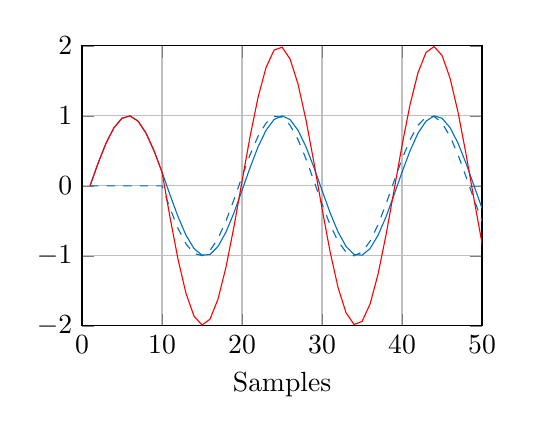
\begin{tikzpicture}

\begin{axis}[%
width=2in,
height=1.4in,
xlabel = {Samples},
%ylabel = {Amplitude}, 
scale only axis,
xmin=0,
xmax=50,
xmajorgrids,
ymin=-2,
ymax=2,
ymajorgrids,
axis background/.style={fill=white}
]
\addplot [color=mycolor1,solid,forget plot]
  table[row sep=crcr]{%
1	0\\
2	0.321439465303162\\
3	0.608761429008721\\
4	0.831469612302545\\
5	0.965925826289068\\
6	0.997858923238603\\
7	0.923879532511287\\
8	0.751839807478978\\
9	0.5\\
10	0.195090322016128\\
11	-0.130526192220051\\
12	-0.442288690219001\\
13	-0.707106781186548\\
14	-0.896872741532688\\
15	-0.99144486137381\\
16	-0.98078528040323\\
17	-0.866025403784439\\
18	-0.659345815100069\\
19	-0.38268343236509\\
20	-0.0654031292301428\\
21	0.25881904510252\\
22	0.555570233019602\\
23	0.793353340291235\\
24	0.946930129495105\\
25	1\\
26	0.946930129495106\\
27	0.793353340291235\\
28	0.555570233019604\\
29	0.258819045102523\\
30	-0.0654031292301431\\
31	-0.38268343236509\\
32	-0.659345815100069\\
33	-0.866025403784438\\
34	-0.98078528040323\\
35	-0.991444861373811\\
36	-0.896872741532689\\
37	-0.707106781186547\\
38	-0.442288690219002\\
39	-0.130526192220051\\
40	0.195090322016127\\
41	0.499999999999999\\
42	0.751839807478976\\
43	0.923879532511286\\
44	0.997858923238604\\
45	0.965925826289069\\
46	0.831469612302546\\
47	0.608761429008723\\
48	0.321439465303162\\
49	-1.16403343982657e-15\\
50	-0.321439465303164\\
51	-0.608761429008723\\
52	-0.831469612302545\\
53	-0.965925826289068\\
54	-0.997858923238603\\
55	-0.923879532511286\\
56	-0.751839807478978\\
57	-0.5\\
58	-0.195090322016128\\
59	0.130526192220052\\
60	0.442288690218998\\
61	0.707106781186548\\
62	0.89687274153269\\
63	0.99144486137381\\
64	0.98078528040323\\
65	0.866025403784438\\
66	0.659345815100069\\
67	0.382683432365093\\
68	0.0654031292301461\\
69	-0.258819045102525\\
70	-0.555570233019603\\
71	-0.793353340291236\\
72	-0.946930129495106\\
73	-1\\
74	-0.946930129495105\\
75	-0.793353340291237\\
76	-0.555570233019604\\
77	-0.25881904510252\\
78	0.0654031292301442\\
79	0.382683432365091\\
80	0.65934581510007\\
81	0.866025403784439\\
82	0.98078528040323\\
83	0.991444861373811\\
84	0.896872741532689\\
85	0.707106781186549\\
86	0.442288690219003\\
87	0.13052619222005\\
88	-0.19509032201613\\
89	-0.499999999999999\\
90	-0.751839807478979\\
91	-0.923879532511286\\
92	-0.997858923238603\\
93	-0.965925826289069\\
94	-0.831469612302548\\
95	-0.608761429008722\\
96	-0.321439465303163\\
97	2.32806687965315e-15\\
};
\addplot [color=mycolor1,dashed,forget plot]
  table[row sep=crcr]{%
1	0\\
2	0\\
3	0\\
4	0\\
5	0\\
6	0\\
7	0\\
8	0\\
9	0\\
10	0\\
11	-0.321439465303162\\
12	-0.608761429008721\\
13	-0.831469612302545\\
14	-0.965925826289068\\
15	-0.997858923238603\\
16	-0.923879532511287\\
17	-0.751839807478978\\
18	-0.5\\
19	-0.195090322016128\\
20	0.130526192220051\\
21	0.442288690219001\\
22	0.707106781186548\\
23	0.896872741532688\\
24	0.99144486137381\\
25	0.98078528040323\\
26	0.866025403784439\\
27	0.659345815100069\\
28	0.38268343236509\\
29	0.0654031292301428\\
30	-0.25881904510252\\
31	-0.555570233019602\\
32	-0.793353340291235\\
33	-0.946930129495105\\
34	-1\\
35	-0.946930129495106\\
36	-0.793353340291235\\
37	-0.555570233019604\\
38	-0.258819045102523\\
39	0.0654031292301431\\
40	0.38268343236509\\
41	0.659345815100069\\
42	0.866025403784438\\
43	0.98078528040323\\
44	0.991444861373811\\
45	0.896872741532689\\
46	0.707106781186547\\
47	0.442288690219002\\
48	0.130526192220051\\
49	-0.195090322016127\\
50	-0.499999999999999\\
51	-0.751839807478976\\
52	-0.923879532511286\\
53	-0.997858923238604\\
54	-0.965925826289069\\
55	-0.831469612302546\\
56	-0.608761429008723\\
57	-0.321439465303162\\
58	1.16403343982657e-15\\
59	0.321439465303164\\
60	0.608761429008723\\
61	0.831469612302545\\
62	0.965925826289068\\
63	0.997858923238603\\
64	0.923879532511286\\
65	0.751839807478978\\
66	0.5\\
67	0.195090322016128\\
68	-0.130526192220052\\
69	-0.442288690218998\\
70	-0.707106781186548\\
71	-0.89687274153269\\
72	-0.99144486137381\\
73	-0.98078528040323\\
74	-0.866025403784438\\
75	-0.659345815100069\\
76	-0.382683432365093\\
77	-0.0654031292301461\\
78	0.258819045102525\\
79	0.555570233019603\\
80	0.793353340291236\\
81	0.946930129495106\\
82	1\\
83	0.946930129495105\\
84	0.793353340291237\\
85	0.555570233019604\\
86	0.25881904510252\\
87	-0.0654031292301442\\
88	-0.382683432365091\\
89	-0.65934581510007\\
90	-0.866025403784439\\
91	-0.98078528040323\\
92	-0.991444861373811\\
93	-0.896872741532689\\
94	-0.707106781186549\\
95	-0.442288690219003\\
96	-0.13052619222005\\
97	0.19509032201613\\
98	0.499999999999999\\
99	0.751839807478979\\
100	0.923879532511286\\
101	0.997858923238603\\
102	0.965925826289069\\
103	0.831469612302548\\
104	0.608761429008722\\
105	0.321439465303163\\
106	-2.32806687965315e-15\\
};
\addplot [color=red,solid,forget plot]
  table[row sep=crcr]{%
1	0\\
2	0.321439465303162\\
3	0.608761429008721\\
4	0.831469612302545\\
5	0.965925826289068\\
6	0.997858923238603\\
7	0.923879532511287\\
8	0.751839807478978\\
9	0.5\\
10	0.195090322016128\\
11	-0.451965657523213\\
12	-1.05105011922772\\
13	-1.53857639348909\\
14	-1.86279856782176\\
15	-1.98930378461241\\
16	-1.90466481291452\\
17	-1.61786521126342\\
18	-1.15934581510007\\
19	-0.577773754381218\\
20	0.0651230629899085\\
21	0.701107735321521\\
22	1.26267701420615\\
23	1.69022608182392\\
24	1.93837499086892\\
25	1.98078528040323\\
26	1.81295553327954\\
27	1.4526991553913\\
28	0.938253665384693\\
29	0.324222174332665\\
30	-0.324222174332663\\
31	-0.938253665384692\\
32	-1.4526991553913\\
33	-1.81295553327954\\
34	-1.98078528040323\\
35	-1.93837499086892\\
36	-1.69022608182392\\
37	-1.26267701420615\\
38	-0.701107735321525\\
39	-0.065123062989908\\
40	0.577773754381217\\
41	1.15934581510007\\
42	1.61786521126341\\
43	1.90466481291452\\
44	1.98930378461241\\
45	1.86279856782176\\
46	1.53857639348909\\
47	1.05105011922773\\
48	0.451965657523213\\
49	-0.195090322016128\\
50	-0.821439465303163\\
51	-1.3606012364877\\
52	-1.75534914481383\\
53	-1.96378474952767\\
54	-1.96378474952767\\
55	-1.75534914481383\\
56	-1.3606012364877\\
57	-0.821439465303162\\
58	-0.195090322016127\\
59	0.451965657523216\\
60	1.05105011922772\\
61	1.53857639348909\\
62	1.86279856782176\\
63	1.98930378461241\\
64	1.90466481291452\\
65	1.61786521126342\\
66	1.15934581510007\\
67	0.577773754381221\\
68	-0.0651230629899055\\
69	-0.701107735321523\\
70	-1.26267701420615\\
71	-1.69022608182393\\
72	-1.93837499086892\\
73	-1.98078528040323\\
74	-1.81295553327954\\
75	-1.45269915539131\\
76	-0.938253665384697\\
77	-0.324222174332666\\
78	0.324222174332669\\
79	0.938253665384694\\
80	1.45269915539131\\
81	1.81295553327955\\
82	1.98078528040323\\
83	1.93837499086892\\
84	1.69022608182393\\
85	1.26267701420615\\
86	0.701107735321523\\
87	0.0651230629899057\\
88	-0.577773754381221\\
89	-1.15934581510007\\
90	-1.61786521126342\\
91	-1.90466481291452\\
92	-1.98930378461241\\
93	-1.86279856782176\\
94	-1.5385763934891\\
95	-1.05105011922772\\
96	-0.451965657523213\\
97	0.195090322016132\\
};
\end{axis}
\end{tikzpicture}%
	 		%\caption{2500 Hz}
	 	\end{center}
		\end{column}
	\end{columns}
\end{frame}





\begin{frame}{Introduction}{Stationary vs non-stationary signals}		
	\begin{itemize}
		\item Conversion delay
	\end{itemize}
\end{frame}




\subsection{Present consumer headphones}
\begin{frame}{Introduction}{Present consumer headphones}
	\begin{itemize}	
	\item How well does the consumer headphones attenuate?
	\begin{columns}
		\begin{column}{0.27\textwidth}
		\begin{itemize}
			\item Denon AH-GC20
			\item Bose QC25 
			\item Bose QC15 	
			\item B\&O H8 	
		\end{itemize}
		\end{column}
		\begin{column}{0.6\textwidth} 
		\begin{itemize}
			\item[] 2.200 kr (2016)
			\item[] 2.799 kr (2016)
			\item[] 2.696 kr (2011)
			\item[] 3.495 kr (2016)
		\end{itemize}
		\end{column}
	\end{columns}
	\end{itemize}			
	\begin{center}
		% This file was created by matlab2tikz.
%
%The latest updates can be retrieved from
%  http://www.mathworks.com/matlabcentral/fileexchange/22022-matlab2tikz-matlab2tikz
%where you can also make suggestions and rate matlab2tikz.
%
\definecolor{mycolor1}{rgb}{0.00000,0.44700,0.74100}%
\definecolor{mycolor2}{rgb}{0.85000,0.32500,0.09800}%
\definecolor{mycolor3}{rgb}{0.92900,0.69400,0.12500}%
\definecolor{mycolor4}{rgb}{0.49400,0.18400,0.55600}%
%
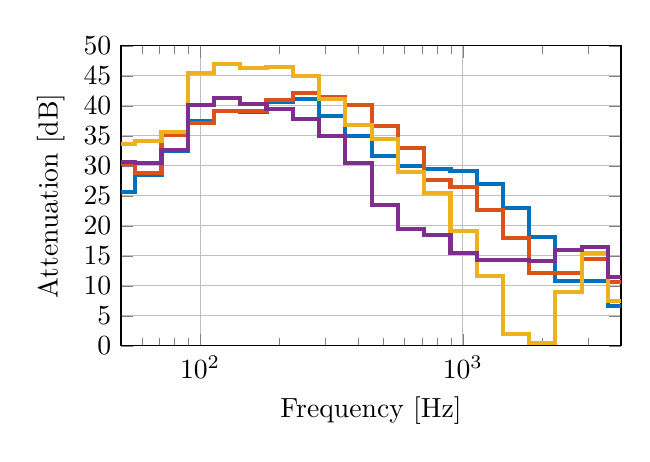
\begin{tikzpicture}

\begin{axis}[%
width=2.5in,
height=1.5in,
at={(1.011in,0.642in)},
scale only axis,
xmode=log,
xmin=50,
xmax=4000,
xlabel={Frequency [Hz]},
xmajorgrids,
%xmajorgrids,
%ymajorgrids,
%xminorgrids,
ymin=0,
ymax=50,
ytick={0,5,...,50},
ylabel={Attenuation [dB]},
ymajorgrids,
axis background/.style={fill=white},
title style={font=\bfseries},
%title={Comparison of Smoothened curves},
legend style={legend cell align=left,align=left,draw=white!15!black}
]
%\addplot[const plot,color=mycolor1,solid,forget plot,thick] plot table[row sep=crcr] {%
%	28.4	15.7\\
%	35.7	15.1\\
%	45	12.4\\
%	56.6	14\\
%	71.3	16.3\\
%	89.7	18.8\\
%	113	19.6\\
%	142	19.5\\
%	179	20.3\\
%	225	20.4\\
%	284	19.2\\
%	357	17.4\\
%	450	15.7\\
%	566	15.1\\
%	713	14.7\\
%	897	14.5\\
%	1.13e+03	13.5\\
%	1.42e+03	11.5\\
%	1.79e+03	9.08\\
%	2.25e+03	5.31\\
%	2.84e+03	5.51\\
%	3.57e+03	3.03\\
%	4.5e+03	2.37\\
%	5.66e+03	2.81\\
%	7.13e+03	3.07\\
%	8.97e+03	3.24\\
%	1.13e+04	1.16\\
%	1.42e+04	0.032\\
%	1.79e+04	0.598\\
%	2e+04	-0.763\\
%};
%\addplot[const plot,color=mycolor2,solid,forget plot,thick] plot table[row sep=crcr] {%
%	28.4	14.7\\
%	35.7	15.3\\
%	45	15.2\\
%	56.6	14.2\\
%	71.3	17.6\\
%	89.7	18.7\\
%	113	19.5\\
%	142	19.5\\
%	179	20.4\\
%	225	21.3\\
%	284	20.8\\
%	357	19.8\\
%	450	18.4\\
%	566	16.5\\
%	713	13.4\\
%	897	13.2\\
%	1.13e+03	11.4\\
%	1.42e+03	8.6\\
%	1.79e+03	6.11\\
%	2.25e+03	6.07\\
%	2.84e+03	7.27\\
%	3.57e+03	4.99\\
%	4.5e+03	2.6\\
%	5.66e+03	2.91\\
%	7.13e+03	1.03\\
%	8.97e+03	2.02\\
%	1.13e+04	-0.338\\
%	1.42e+04	-0.849\\
%	1.79e+04	-0.618\\
%	2e+04	-2.19\\
%};
%\addplot[const plot,color=mycolor3,solid,forget plot,thick] plot table[row sep=crcr] {%
%	28.4	18.1\\
%	35.7	19\\
%	45	17.1\\
%	56.6	16.5\\
%	71.3	18.6\\
%	89.7	22.8\\
%	113	23.6\\
%	142	23.3\\
%	179	23.5\\
%	225	22.6\\
%	284	20.4\\
%	357	18.4\\
%	450	17.2\\
%	566	14.5\\
%	713	12.7\\
%	897	9.48\\
%	1.13e+03	5.89\\
%	1.42e+03	1.04\\
%	1.79e+03	0.132\\
%	2.25e+03	4.45\\
%	2.84e+03	7.76\\
%	3.57e+03	3.73\\
%	4.5e+03	2.58\\
%	5.66e+03	2.46\\
%	7.13e+03	1.18\\
%	8.97e+03	1.16\\
%	1.13e+04	0.0281\\
%	1.42e+04	-0.34\\
%	1.79e+04	-0.623\\
%	2e+04	-1.08\\
%};
%\addplot[const plot,color=mycolor4,solid,forget plot,thick] plot table[row sep=crcr] {%
%	28.4	18.6\\
%	35.7	16.5\\
%	45	15.5\\
%	56.6	15.5\\
%	71.3	16.6\\
%	89.7	20.3\\
%	113	20.4\\
%	142	20\\
%	179	19.6\\
%	225	18.9\\
%	284	17.4\\
%	357	15.3\\
%	450	11.8\\
%	566	9.77\\
%	713	8.89\\
%	897	7.71\\
%	1.13e+03	6.86\\
%	1.42e+03	7.05\\
%	1.79e+03	7.37\\
%	2.25e+03	7.85\\
%	2.84e+03	8.24\\
%	3.57e+03	5.7\\
%	4.5e+03	3.78\\
%	5.66e+03	3.02\\
%	7.13e+03	1.43\\
%	8.97e+03	1.33\\
%	1.13e+04	1.58\\
%	1.42e+04	0.0462\\
%	1.79e+04	-1.02\\
%	2e+04	-0.621\\
%};
%\end{axis}

%% 20 log
\addplot[const plot,color=mycolor1,solid,line width=1.5pt,forget plot] plot table[row sep=crcr] {%
	28.4	30.6\\
	35.7	31.3\\
	45	25.7\\
	56.6	28.5\\
	71.3	32.4\\
	89.7	37.4\\
	113	39.1\\
	142	39\\
	179	40.6\\
	225	41.2\\
	284	38.3\\
	357	35\\
	450	31.7\\
	566	30\\
	713	29.4\\
	897	29.1\\
	1.13e+03	27\\
	1.42e+03	23\\
	1.79e+03	18.2\\
	2.25e+03	10.8\\
	2.84e+03	10.8\\
	3.57e+03	6.62\\
	4.5e+03	4.92\\
	5.66e+03	5.21\\
	7.13e+03	5.95\\
	8.97e+03	5.98\\
	1.13e+04	2.27\\
	1.42e+04	-1\\
	1.79e+04	0.842\\
	2e+04	-1.38\\
};
\addplot[const plot,color=mycolor2,solid,line width=1.5pt,forget plot] plot table[row sep=crcr] {%
	28.4	29.3\\
	35.7	30.1\\
	45	30.3\\
	56.6	28.8\\
	71.3	35.2\\
	89.7	37.2\\
	113	39.1\\
	142	39.2\\
	179	41\\
	225	42.2\\
	284	41.5\\
	357	40.1\\
	450	36.7\\
	566	33\\
	713	27.7\\
	897	26.5\\
	1.13e+03	22.7\\
	1.42e+03	17.9\\
	1.79e+03	12.1\\
	2.25e+03	12.1\\
	2.84e+03	14.4\\
	3.57e+03	10.6\\
	4.5e+03	5.72\\
	5.66e+03	5.17\\
	7.13e+03	2.13\\
	8.97e+03	4.17\\
	1.13e+04	-0.138\\
	1.42e+04	-0.907\\
	1.79e+04	-1.96\\
	2e+04	-4.33\\
};
\addplot[const plot,color=mycolor3,solid,line width=1.5pt,forget plot] plot table[row sep=crcr] {%
	28.4	36.2\\
	35.7	38.5\\
	45	33.6\\
	56.6	34.2\\
	71.3	35.6\\
	89.7	45.5\\
	113	46.9\\
	142	46.3\\
	179	46.5\\
	225	44.9\\
	284	41.1\\
	357	36.8\\
	450	34.5\\
	566	29\\
	713	25.5\\
	897	19.1\\
	1.13e+03	11.6\\
	1.42e+03	1.91\\
	1.79e+03	0.429\\
	2.25e+03	9.03\\
	2.84e+03	15.5\\
	3.57e+03	7.47\\
	4.5e+03	4.95\\
	5.66e+03	4.31\\
	7.13e+03	2.18\\
	8.97e+03	2.87\\
	1.13e+04	0.264\\
	1.42e+04	-0.554\\
	1.79e+04	-2.08\\
	2e+04	-2.36\\
};
\addplot[const plot,color=mycolor4,solid,line width=1.5pt,forget plot] plot table[row sep=crcr] {%
	28.4	37.2\\
	35.7	33.9\\
	45	30.7\\
	56.6	30.4\\
	71.3	32.7\\
	89.7	40.2\\
	113	41.3\\
	142	40.3\\
	179	39.5\\
	225	37.8\\
	284	34.9\\
	357	30.5\\
	450	23.4\\
	566	19.5\\
	713	18.4\\
	897	15.4\\
	1.13e+03	14.3\\
	1.42e+03	14.3\\
	1.79e+03	14.1\\
	2.25e+03	16\\
	2.84e+03	16.4\\
	3.57e+03	11.5\\
	4.5e+03	7.26\\
	5.66e+03	6.34\\
	7.13e+03	2.99\\
	8.97e+03	2.87\\
	1.13e+04	2.9\\
	1.42e+04	0.784\\
	1.79e+04	-1.51\\
	2e+04	-1.74\\
};
\end{axis}
\end{tikzpicture}%
	\end{center}	
\end{frame}





\begin{frame}{Introduction}{A solution for the problem}		
	\begin{itemize}
		\item Conversion delay
	\end{itemize}
\end{frame}


\section{Methods}







\subsection{Adaptive Filtered-x least mean squares FIR algorithm}

\subsection{Wiener filtering}

\section{Results}

\subsection{Simulation}


\section{Discussion}

\subsection{Computation}

\section{Conclusion}

\subsection{Listen}
